% Options for packages loaded elsewhere
\PassOptionsToPackage{unicode}{hyperref}
\PassOptionsToPackage{hyphens}{url}
%
\documentclass[
  ignorenonframetext,
]{beamer}
\usepackage{pgfpages}
\setbeamertemplate{caption}[numbered]
\setbeamertemplate{caption label separator}{: }
\setbeamercolor{caption name}{fg=normal text.fg}
\beamertemplatenavigationsymbolsempty
% Prevent slide breaks in the middle of a paragraph
\widowpenalties 1 10000
\raggedbottom
\setbeamertemplate{part page}{
  \centering
  \begin{beamercolorbox}[sep=16pt,center]{part title}
    \usebeamerfont{part title}\insertpart\par
  \end{beamercolorbox}
}
\setbeamertemplate{section page}{
  \centering
  \begin{beamercolorbox}[sep=12pt,center]{part title}
    \usebeamerfont{section title}\insertsection\par
  \end{beamercolorbox}
}
\setbeamertemplate{subsection page}{
  \centering
  \begin{beamercolorbox}[sep=8pt,center]{part title}
    \usebeamerfont{subsection title}\insertsubsection\par
  \end{beamercolorbox}
}
\AtBeginPart{
  \frame{\partpage}
}
\AtBeginSection{
  \ifbibliography
  \else
    \frame{\sectionpage}
  \fi
}
\AtBeginSubsection{
  \frame{\subsectionpage}
}
\usepackage{amsmath,amssymb}
\usepackage{lmodern}
\usepackage{iftex}
\ifPDFTeX
  \usepackage[T1]{fontenc}
  \usepackage[utf8]{inputenc}
  \usepackage{textcomp} % provide euro and other symbols
\else % if luatex or xetex
  \usepackage{unicode-math}
  \defaultfontfeatures{Scale=MatchLowercase}
  \defaultfontfeatures[\rmfamily]{Ligatures=TeX,Scale=1}
\fi
\usetheme[]{default}
\usefonttheme{professionalfonts}
% Use upquote if available, for straight quotes in verbatim environments
\IfFileExists{upquote.sty}{\usepackage{upquote}}{}
\IfFileExists{microtype.sty}{% use microtype if available
  \usepackage[]{microtype}
  \UseMicrotypeSet[protrusion]{basicmath} % disable protrusion for tt fonts
}{}
\makeatletter
\@ifundefined{KOMAClassName}{% if non-KOMA class
  \IfFileExists{parskip.sty}{%
    \usepackage{parskip}
  }{% else
    \setlength{\parindent}{0pt}
    \setlength{\parskip}{6pt plus 2pt minus 1pt}}
}{% if KOMA class
  \KOMAoptions{parskip=half}}
\makeatother
\usepackage{xcolor}
\newif\ifbibliography
\usepackage{graphicx}
\makeatletter
\def\maxwidth{\ifdim\Gin@nat@width>\linewidth\linewidth\else\Gin@nat@width\fi}
\def\maxheight{\ifdim\Gin@nat@height>\textheight\textheight\else\Gin@nat@height\fi}
\makeatother
% Scale images if necessary, so that they will not overflow the page
% margins by default, and it is still possible to overwrite the defaults
% using explicit options in \includegraphics[width, height, ...]{}
\setkeys{Gin}{width=\maxwidth,height=\maxheight,keepaspectratio}
% Set default figure placement to htbp
\makeatletter
\def\fps@figure{htbp}
\makeatother
\setlength{\emergencystretch}{3em} % prevent overfull lines
\providecommand{\tightlist}{%
  \setlength{\itemsep}{0pt}\setlength{\parskip}{0pt}}
\setcounter{secnumdepth}{-\maxdimen} % remove section numbering
\usepackage{fancyhdr}
\usepackage{lastpage}
% \setbeamertemplate{navigation symbols}{}
\setbeamertemplate{footline}[page number]
\pagenumbering{arabic}
% \usepackage[mathbf,mathcal,text-hat-accent]{euler}
\ifLuaTeX
  \usepackage{selnolig}  % disable illegal ligatures
\fi
\IfFileExists{bookmark.sty}{\usepackage{bookmark}}{\usepackage{hyperref}}
\IfFileExists{xurl.sty}{\usepackage{xurl}}{} % add URL line breaks if available
\urlstyle{same} % disable monospaced font for URLs
\hypersetup{
  hidelinks,
  pdfcreator={LaTeX via pandoc}}

\title{Diseños de regresión discontinua}
\author{Diseño e implementación de experimentos en ciencias sociales\\
\emph{Departamento de Economía (UdelaR)}}
\date{}

\begin{document}
\frame{\titlepage}

\hypertarget{regresiuxf3n-discontinua-motivaciuxf3n}{%
\section{Regresión Discontinua:
motivación}\label{regresiuxf3n-discontinua-motivaciuxf3n}}

\begin{frame}{Motivación}
\protect\hypertarget{motivaciuxf3n}{}
Objetivo: efecto causal de un programa de becas sobre rendimiento
académico de los estudiantes

Mecanismo de asignación:

\begin{itemize}
\tightlist
\item
  Postulantes toman un examen, reciben un puntaje \(X\)
\item
  Las becas son asignadas a los que obtienen \(X>=c\)
\end{itemize}

Diferencias en rendimiento académico entre estudiantes por encima y por
debajo de \(c\)

\begin{enumerate}
\tightlist
\item
  Efecto causal de la beca
\item
  \emph{Confounders}: IQ, horas de estudio, motivación, características
  del hogar, etc.,\ldots{}
\end{enumerate}
\end{frame}

\begin{frame}{Motivación}
\protect\hypertarget{motivaciuxf3n-1}{}
\begin{itemize}
\item
  Muchos de factores de auto-selección (\emph{counfounding}) son
  no-observables
\item
  Problema fundamental de superposición entre tratados y controles
\item
  DRD explotan el mecanismo discontinuo de asignación
\item
  Suponemos:

  \begin{enumerate}
  \tightlist
  \item
    Estudiantes no tienen control exacto sobre su puntaje
  \item
    Los inobservables no ``saltan'' en el punto de corte (\emph{cutoff})
  \end{enumerate}
\end{itemize}
\end{frame}

\hypertarget{notaciuxf3n-y-estructura}{%
\section{Notación y estructura}\label{notaciuxf3n-y-estructura}}

\begin{frame}{DRD notación y estructura}
\protect\hypertarget{drd-notaciuxf3n-y-estructura}{}
\begin{itemize}
\item
  Resultados potenciales: (\(Y_{i1},Y_{i0}\)), con
  \(\tau_i =Y_{i1} - Y_{i0}\)
\item
  Variable continua \(X\) (puntaje)
\item
  Indicador de tratamiento: \(T_i = T_i(X_i) = 1\) si es tratado, 0 de
  lo contrario
\item
  Resultado observado: \(Y_i = Y_{i1}T_i + Y_{i0}(1 - T_i)\)
\item
  RD explota una discontinuidad en \(P[T_i = 1 | X_i]\) en algún punto
  de corte \(c\)
\item
  Diseño nítido: \(P[T_i = 1 | X_i] = 1(X_i >= c)\)
\end{itemize}
\end{frame}

\begin{frame}{DRD intuición}
\protect\hypertarget{drd-intuiciuxf3n}{}
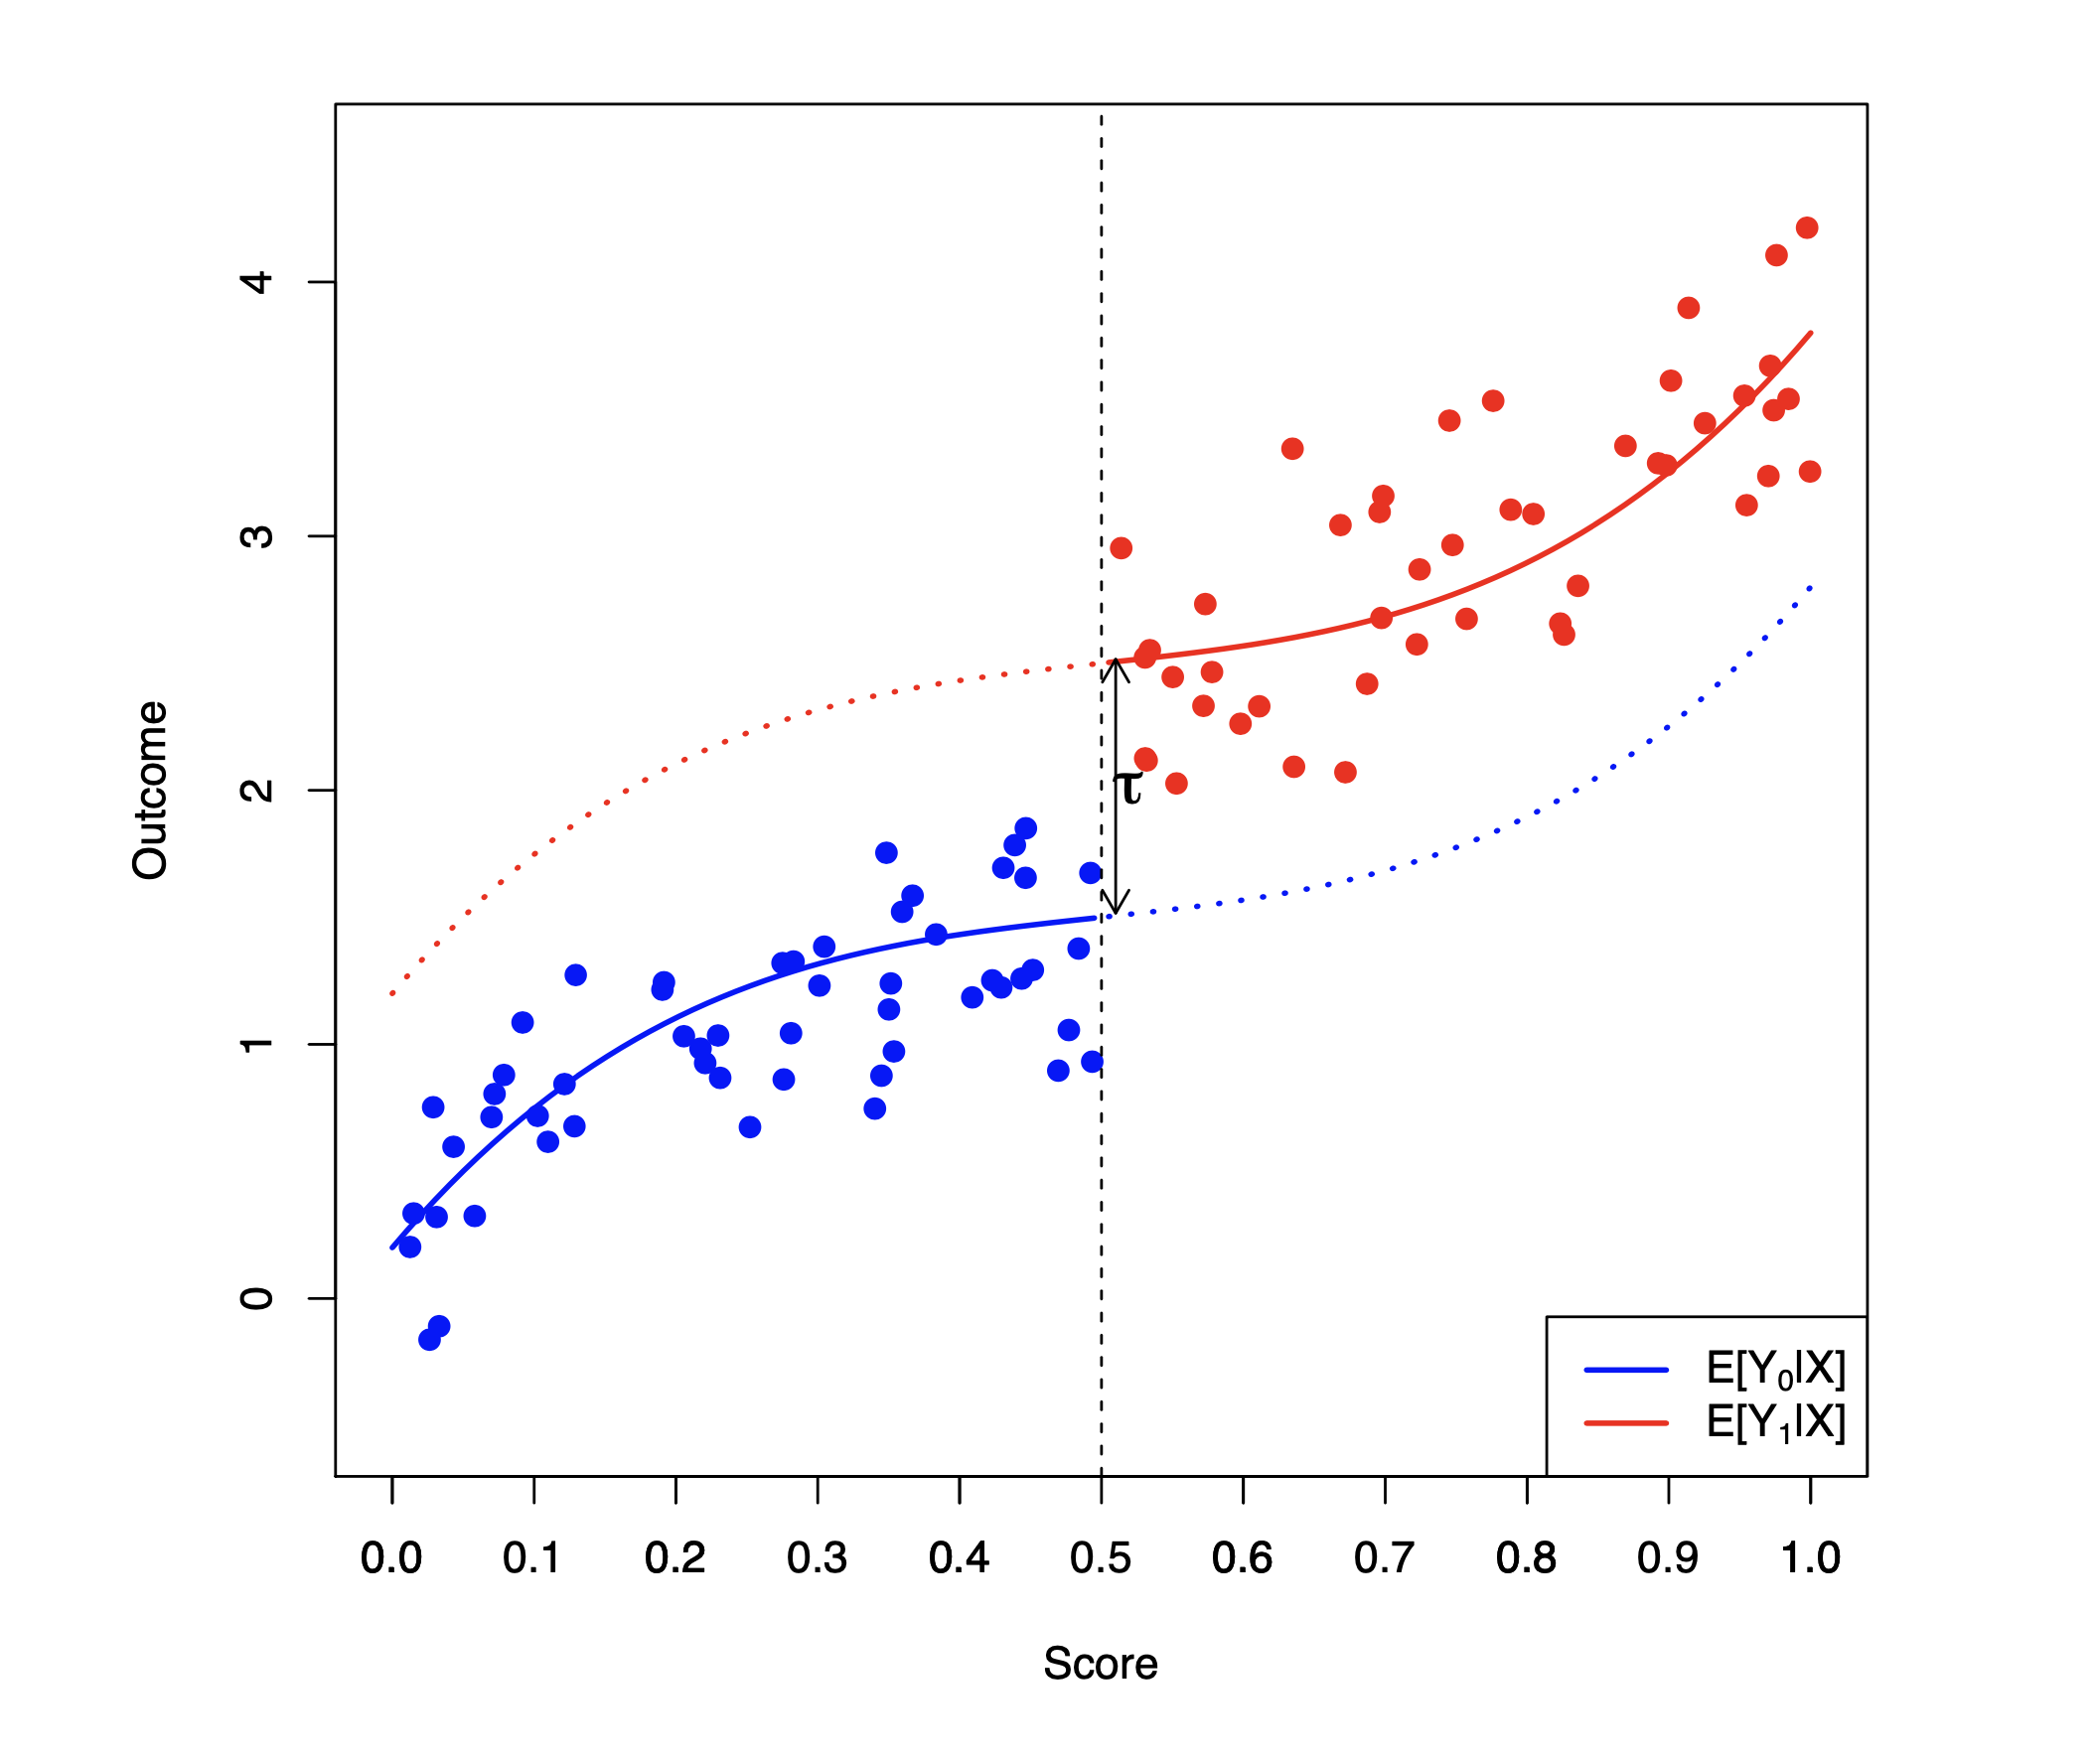
\includegraphics[width=0.9\textwidth,height=\textheight]{rd1}
\end{frame}

\begin{frame}{DRD intuición}
\protect\hypertarget{drd-intuiciuxf3n-1}{}
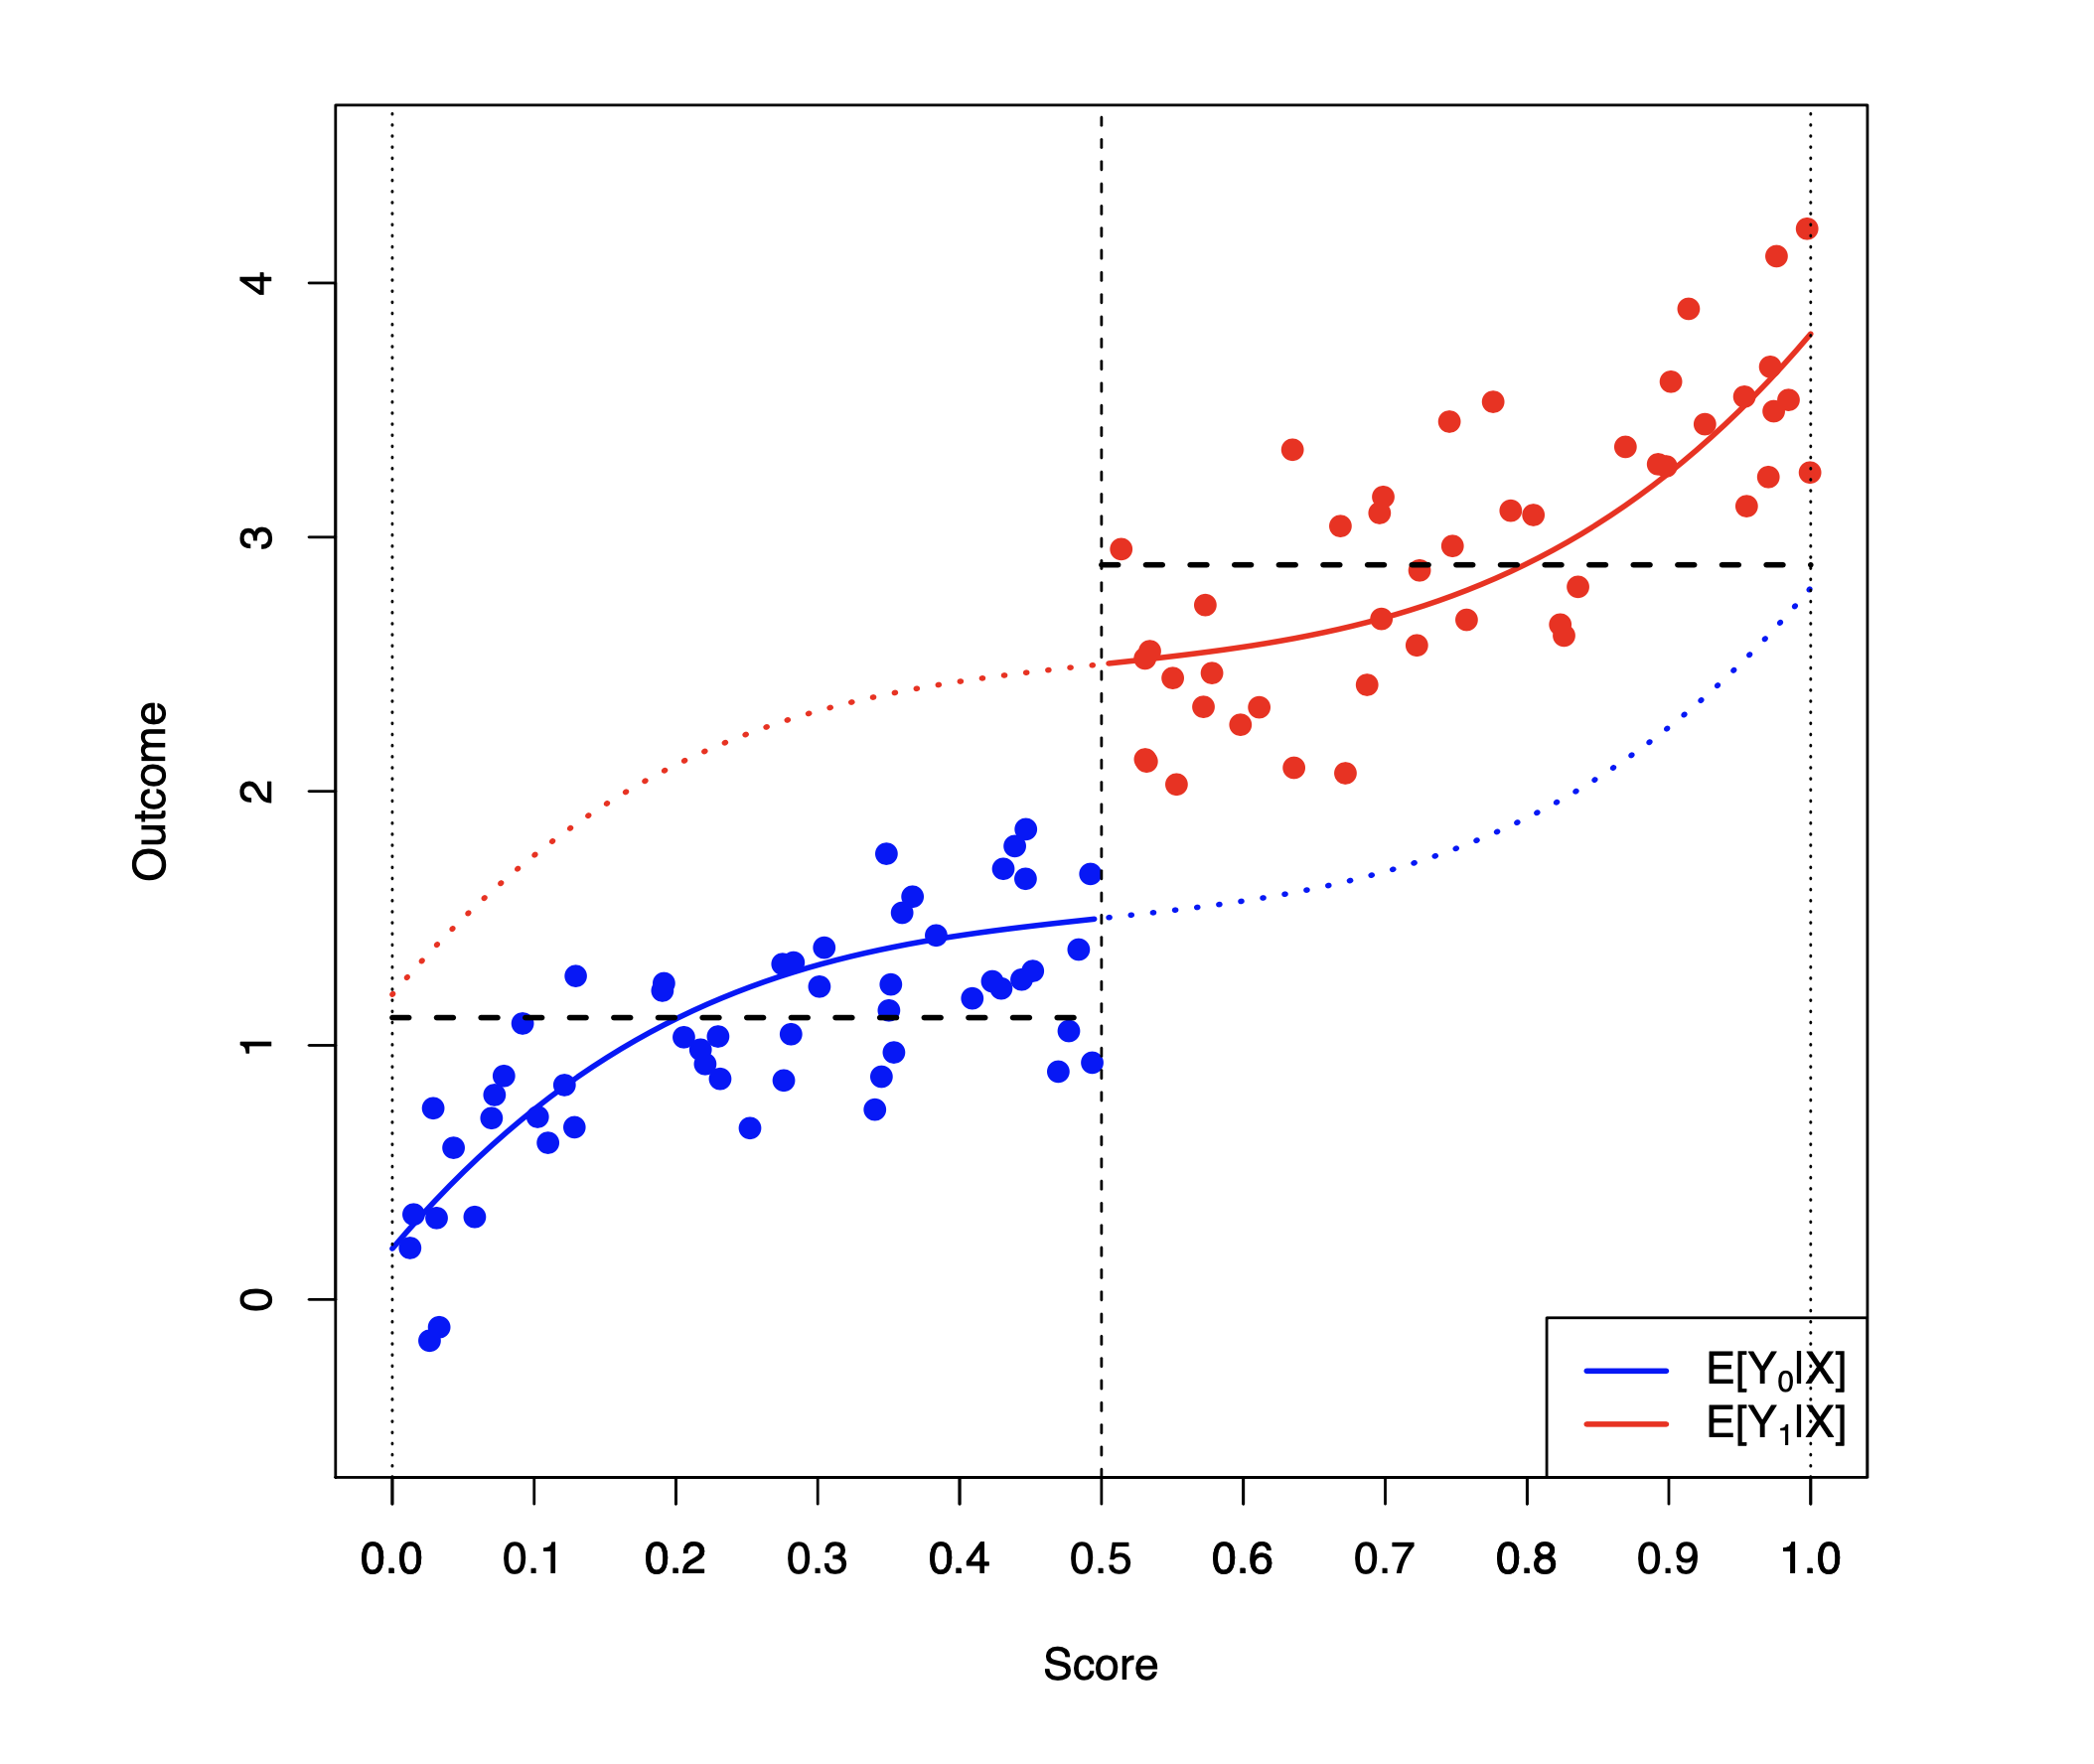
\includegraphics[width=0.9\textwidth,height=\textheight]{rd2}
\end{frame}

\begin{frame}{DRD intuición}
\protect\hypertarget{drd-intuiciuxf3n-2}{}
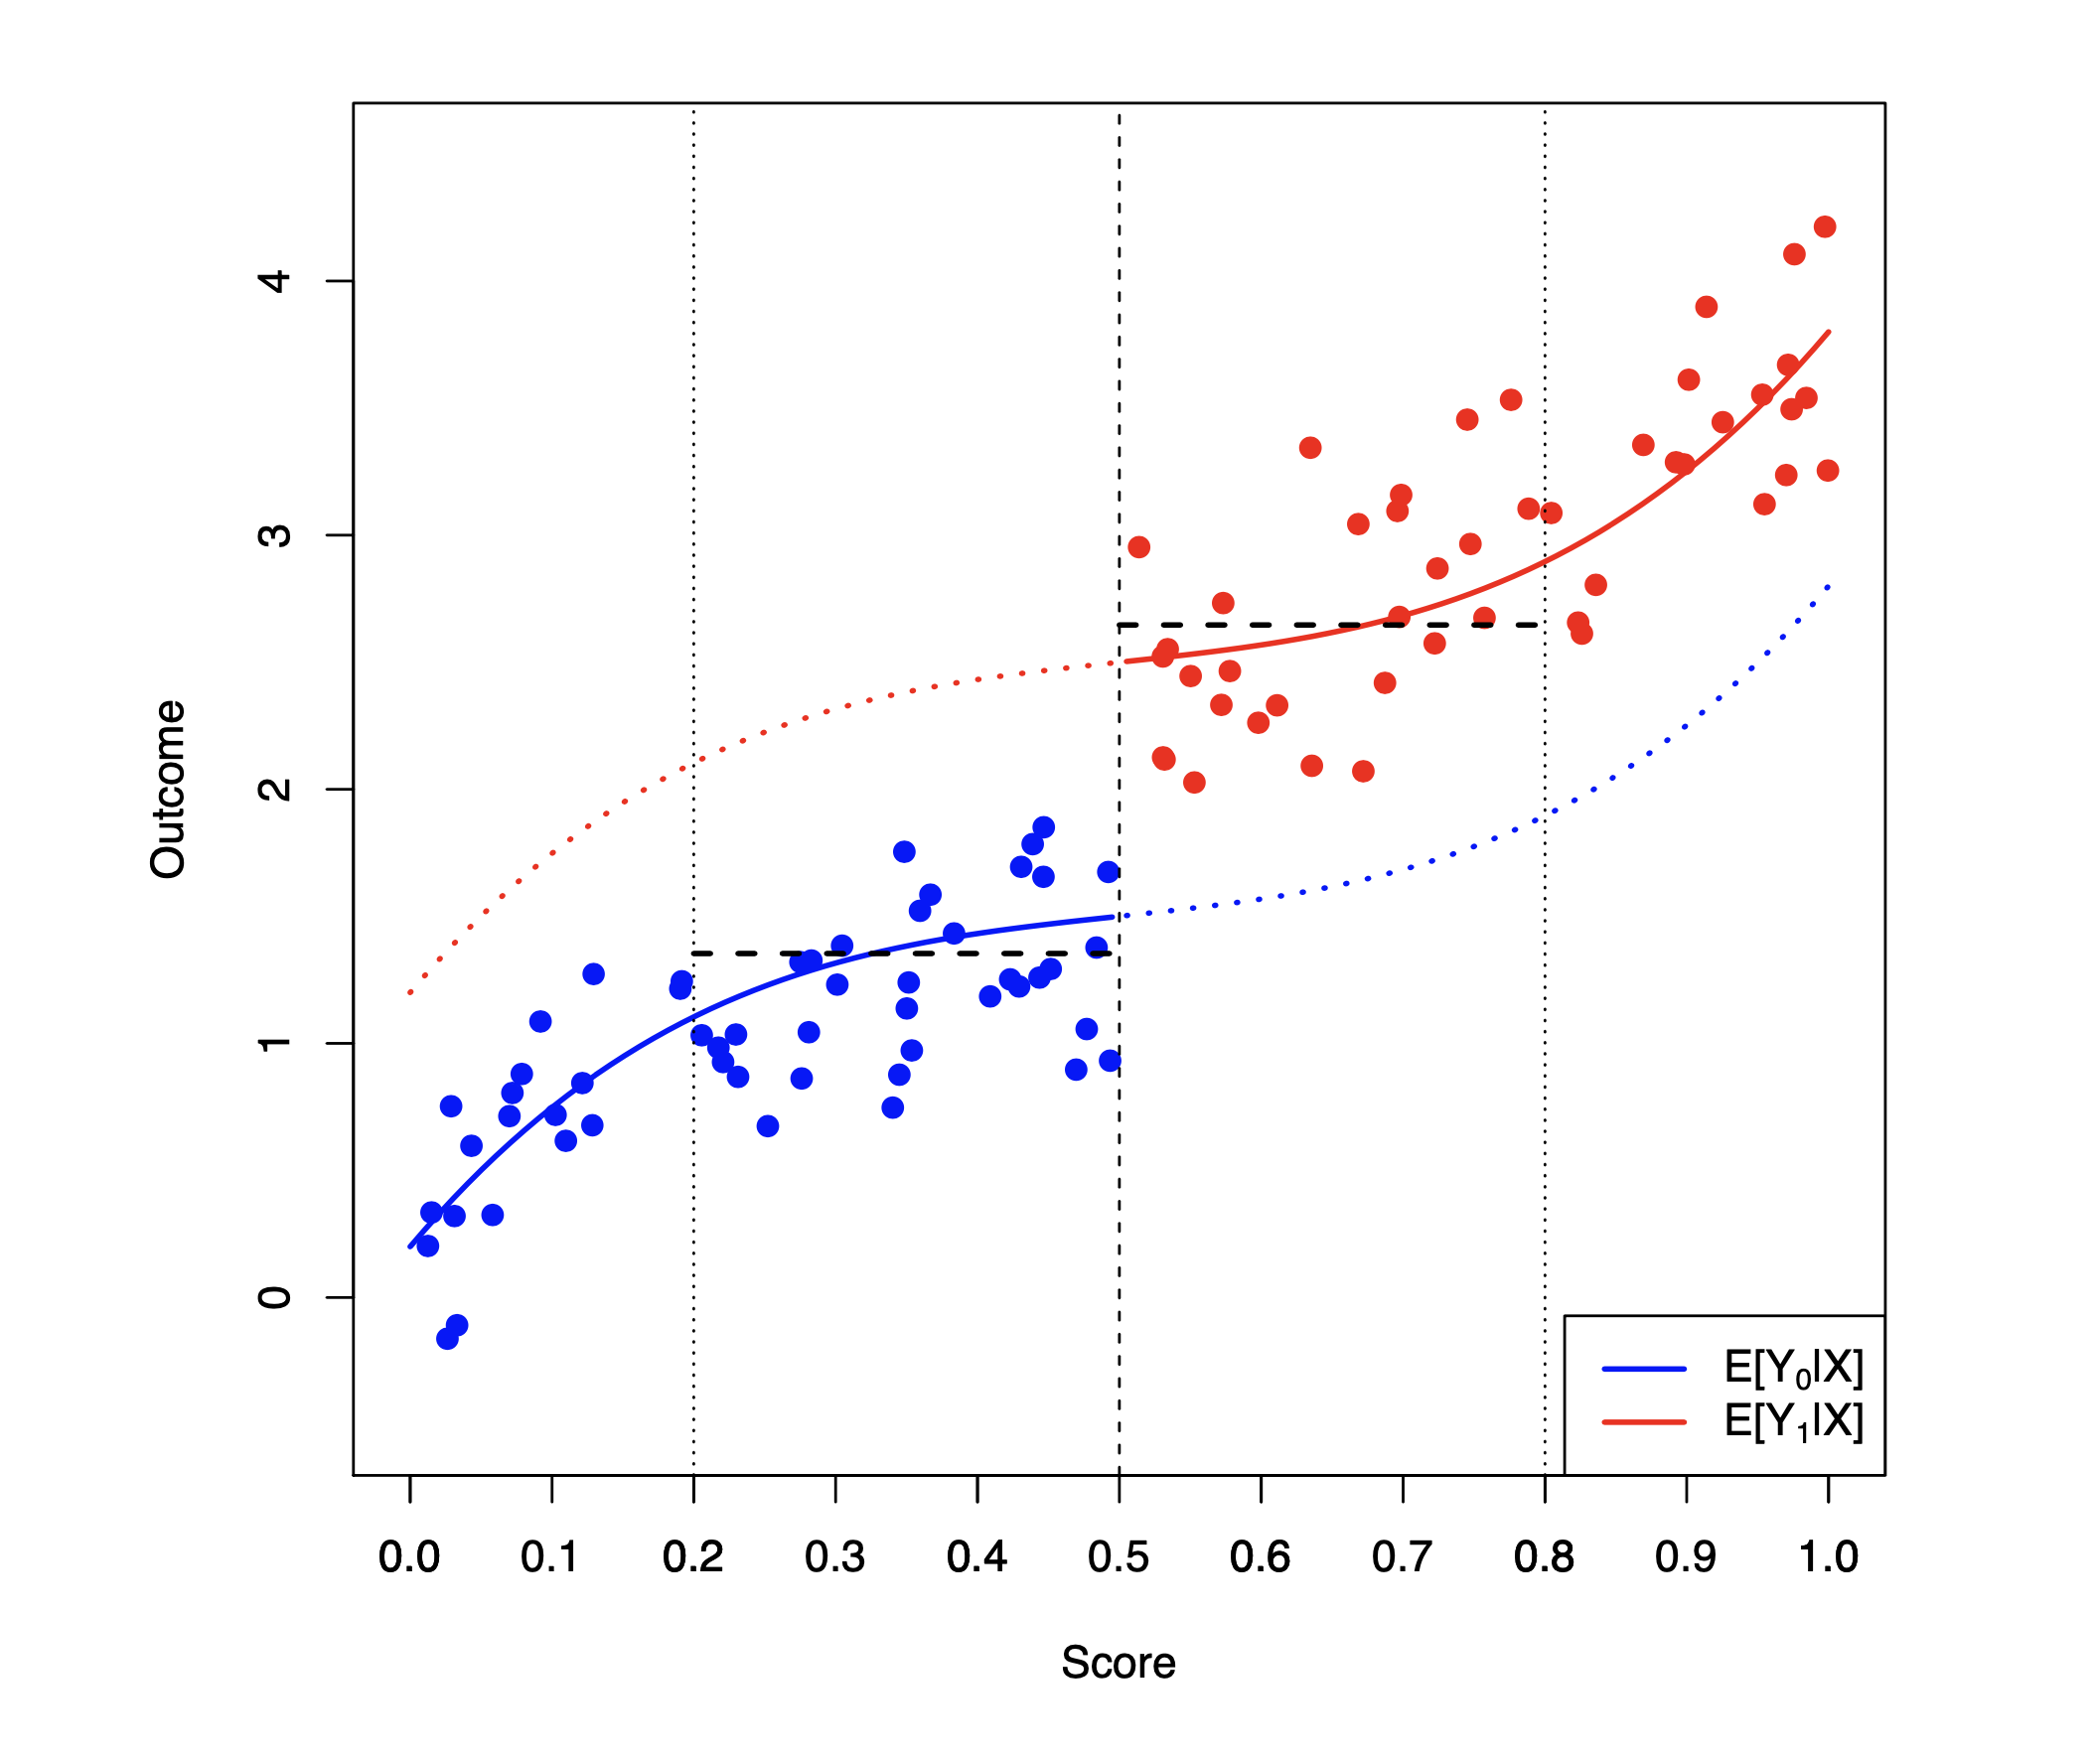
\includegraphics[width=0.9\textwidth,height=\textheight]{rd3}
\end{frame}

\begin{frame}{DRD intuición}
\protect\hypertarget{drd-intuiciuxf3n-3}{}
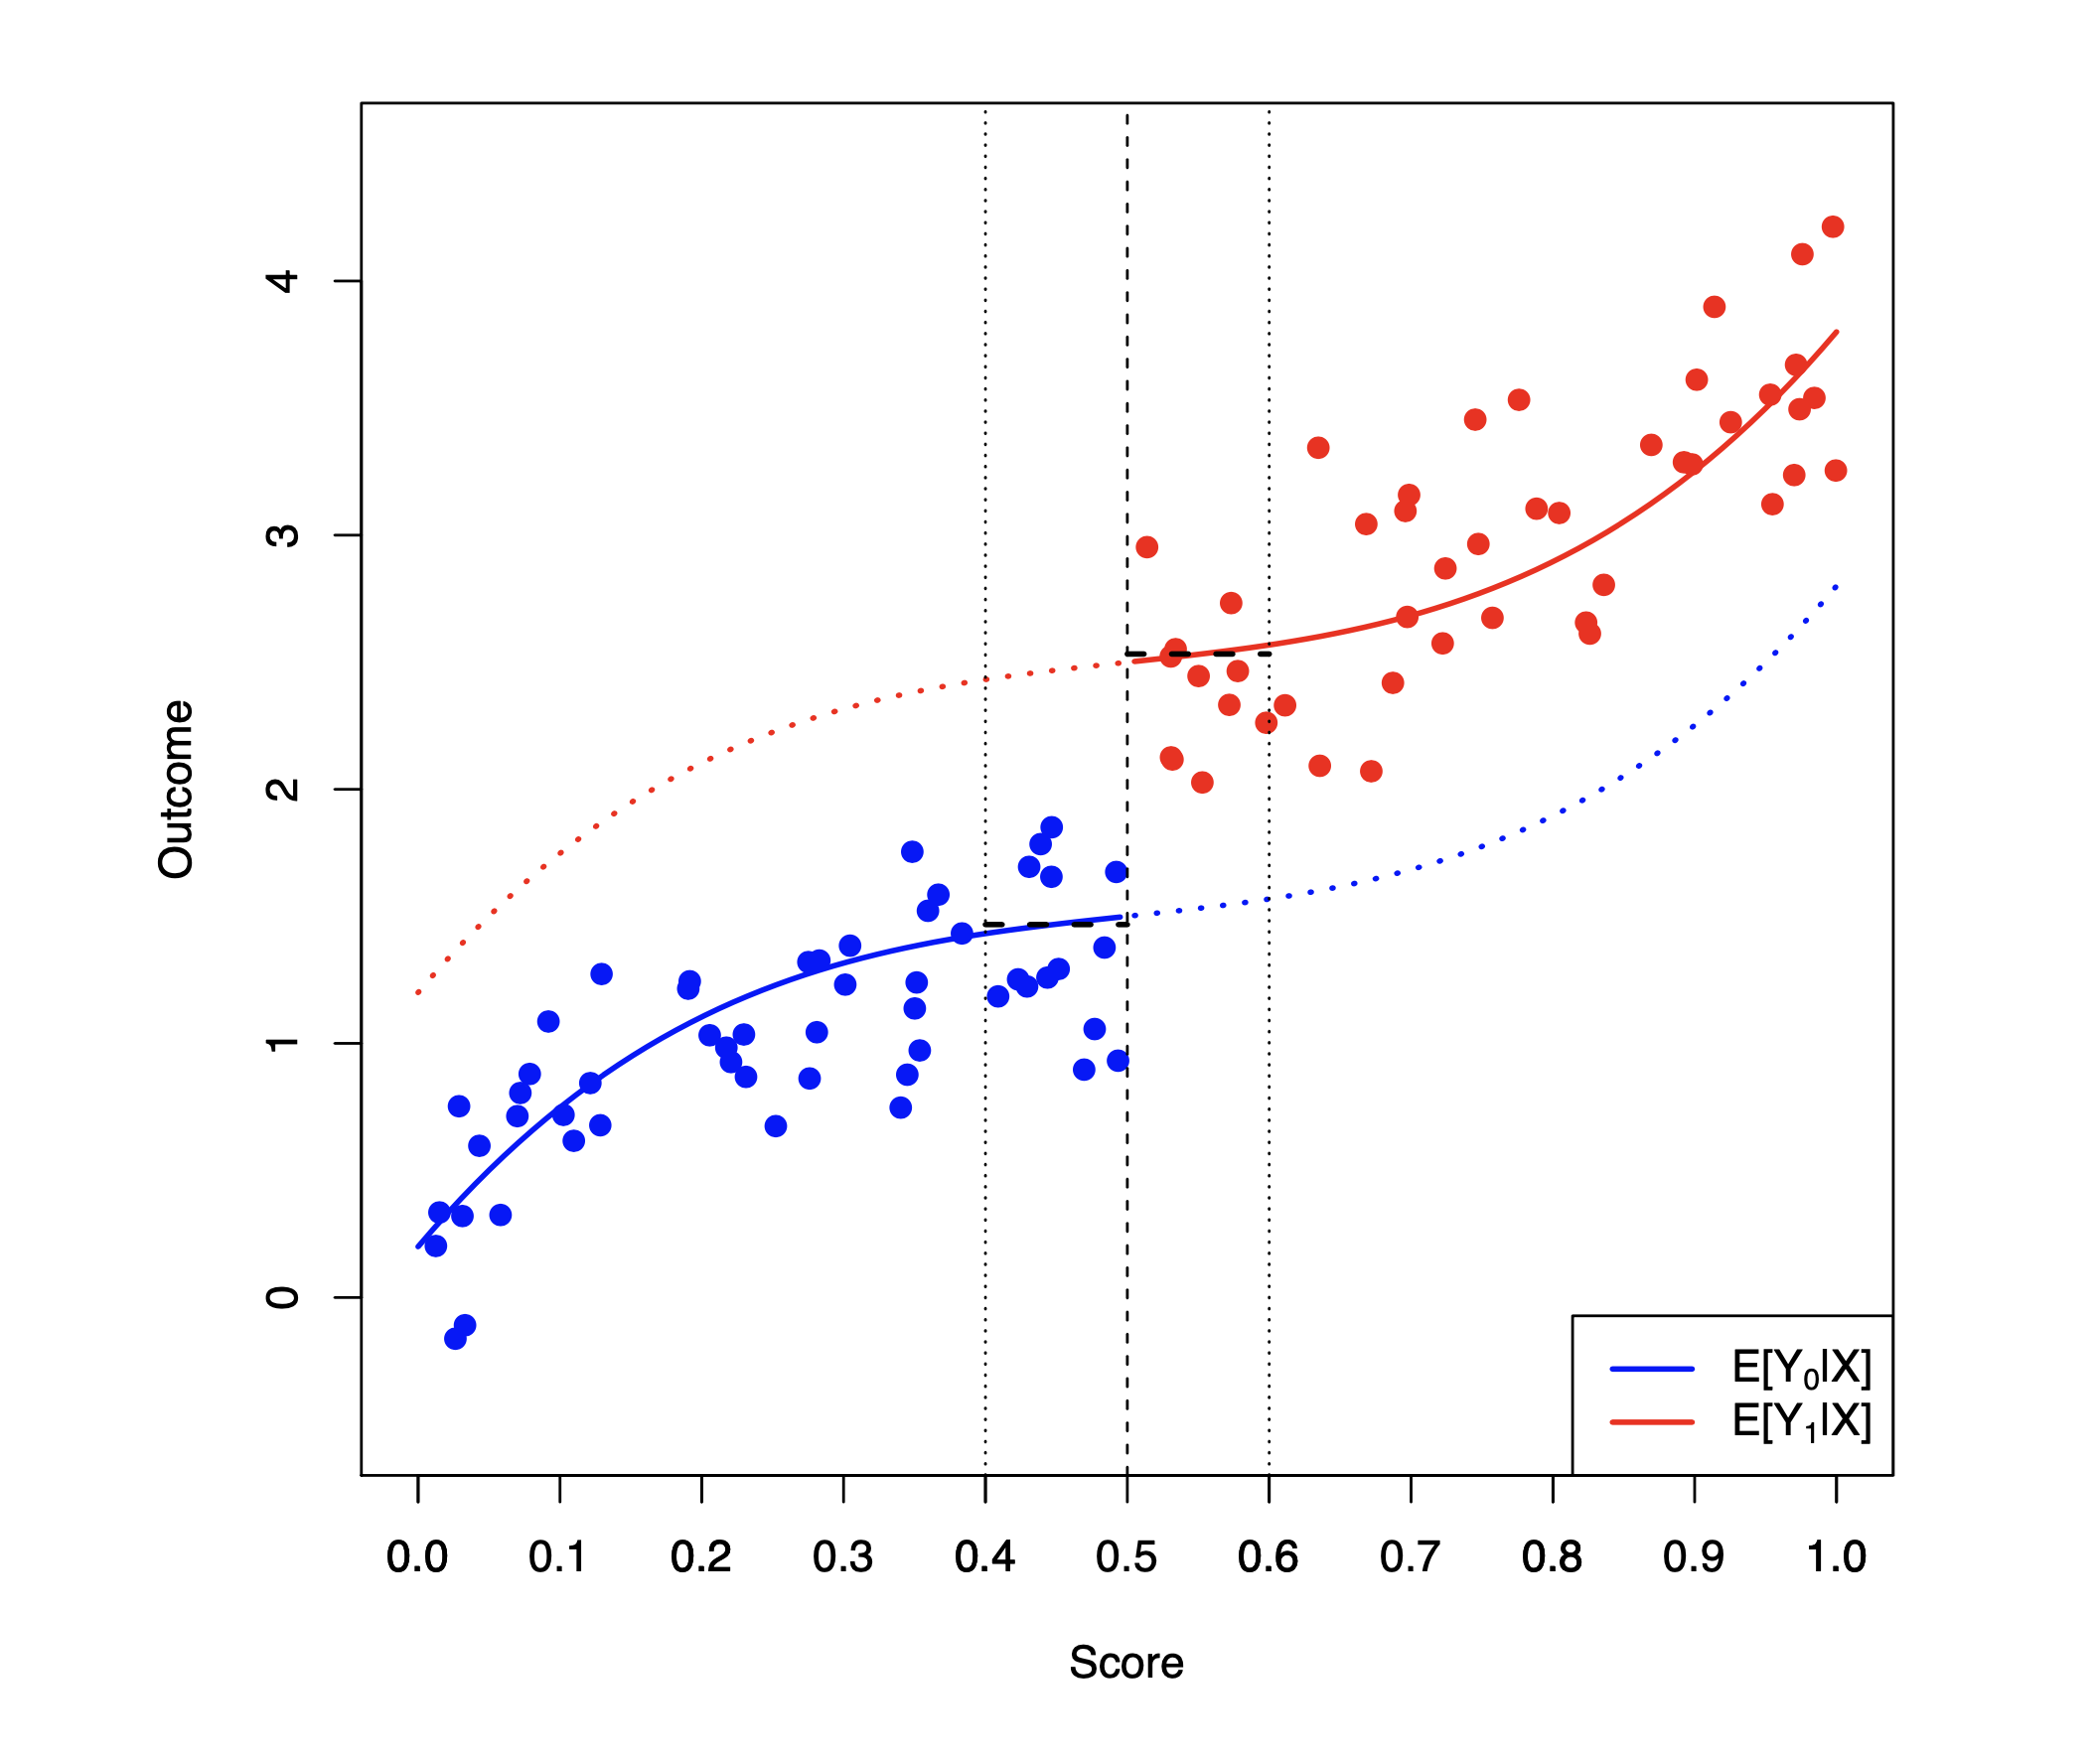
\includegraphics[width=0.9\textwidth,height=\textheight]{rd4}
\end{frame}

\begin{frame}{DRD intuición}
\protect\hypertarget{drd-intuiciuxf3n-4}{}
\begin{itemize}
\tightlist
\item
  Efecto del tratamiento solo se identifica en el punto (\emph{no
  paramétrico})

  \begin{itemize}
  \tightlist
  \item
    Único punto de superposición (en el límite)
  \item
    Interpretación local de la RD
  \end{itemize}
\item
  Estimación en puntos lmítrofes

  \begin{itemize}
  \tightlist
  \item
    En realidad tenemos cero observaciones en \(X_i = c\)
  \item
    Tenemos que basarnos en extrapolación
  \item
    El modelo generalmente está mal especificado
  \end{itemize}
\end{itemize}
\end{frame}

\begin{frame}{DRD ejemplo}
\protect\hypertarget{drd-ejemplo}{}
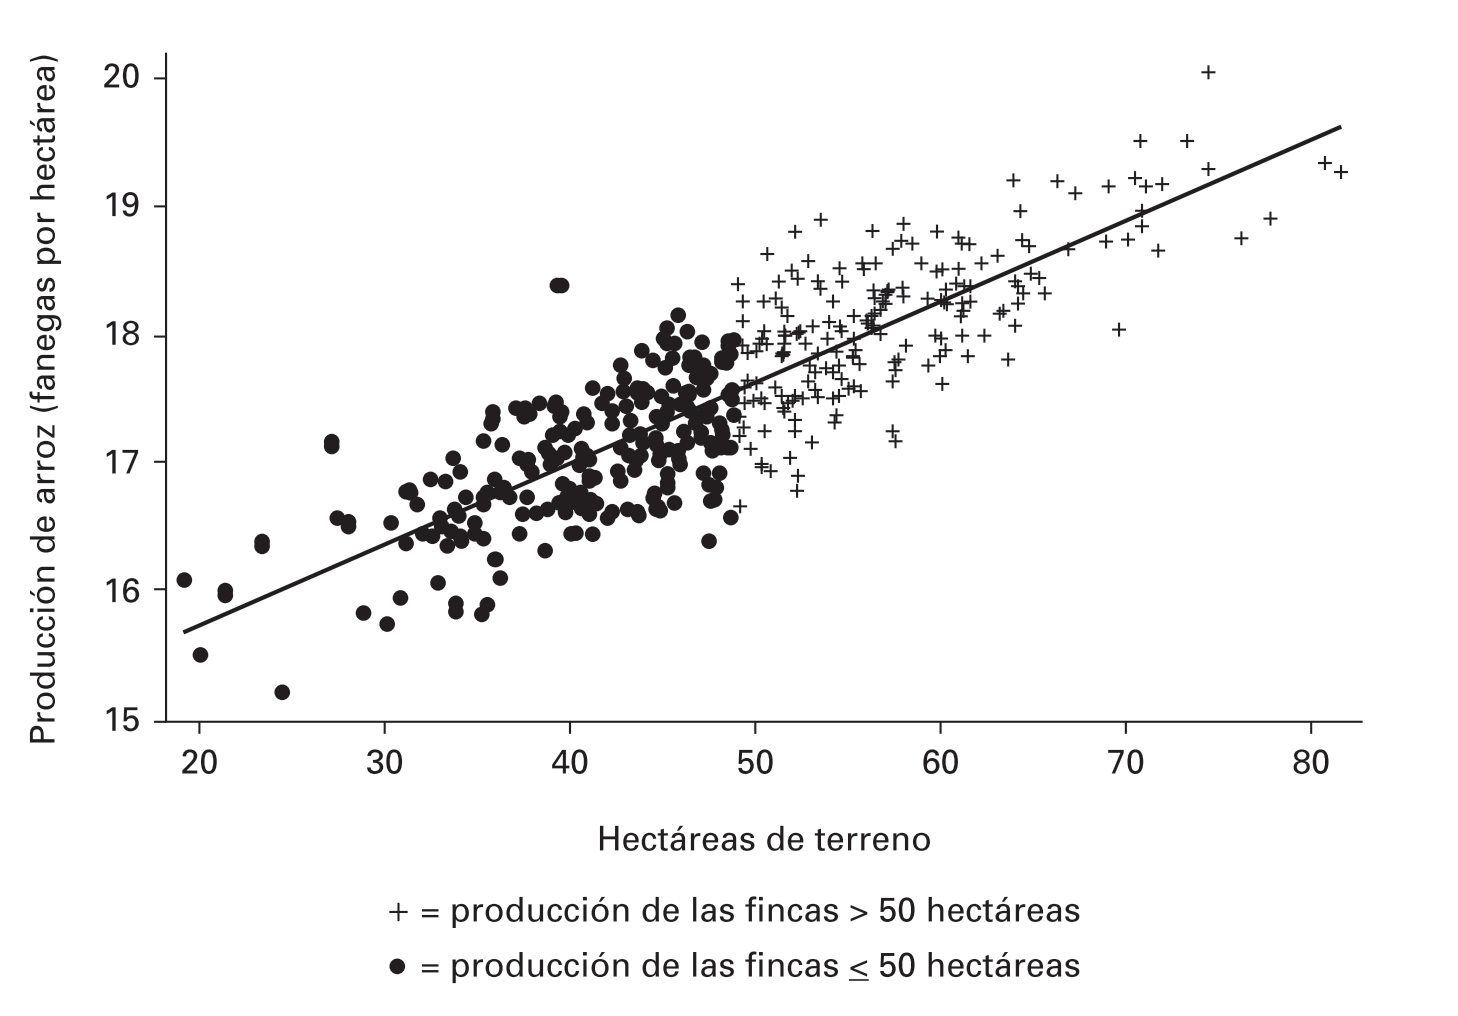
\includegraphics[width=0.9\textwidth,height=\textheight]{arroz}
\end{frame}

\begin{frame}{DRD ejemplo}
\protect\hypertarget{drd-ejemplo-1}{}
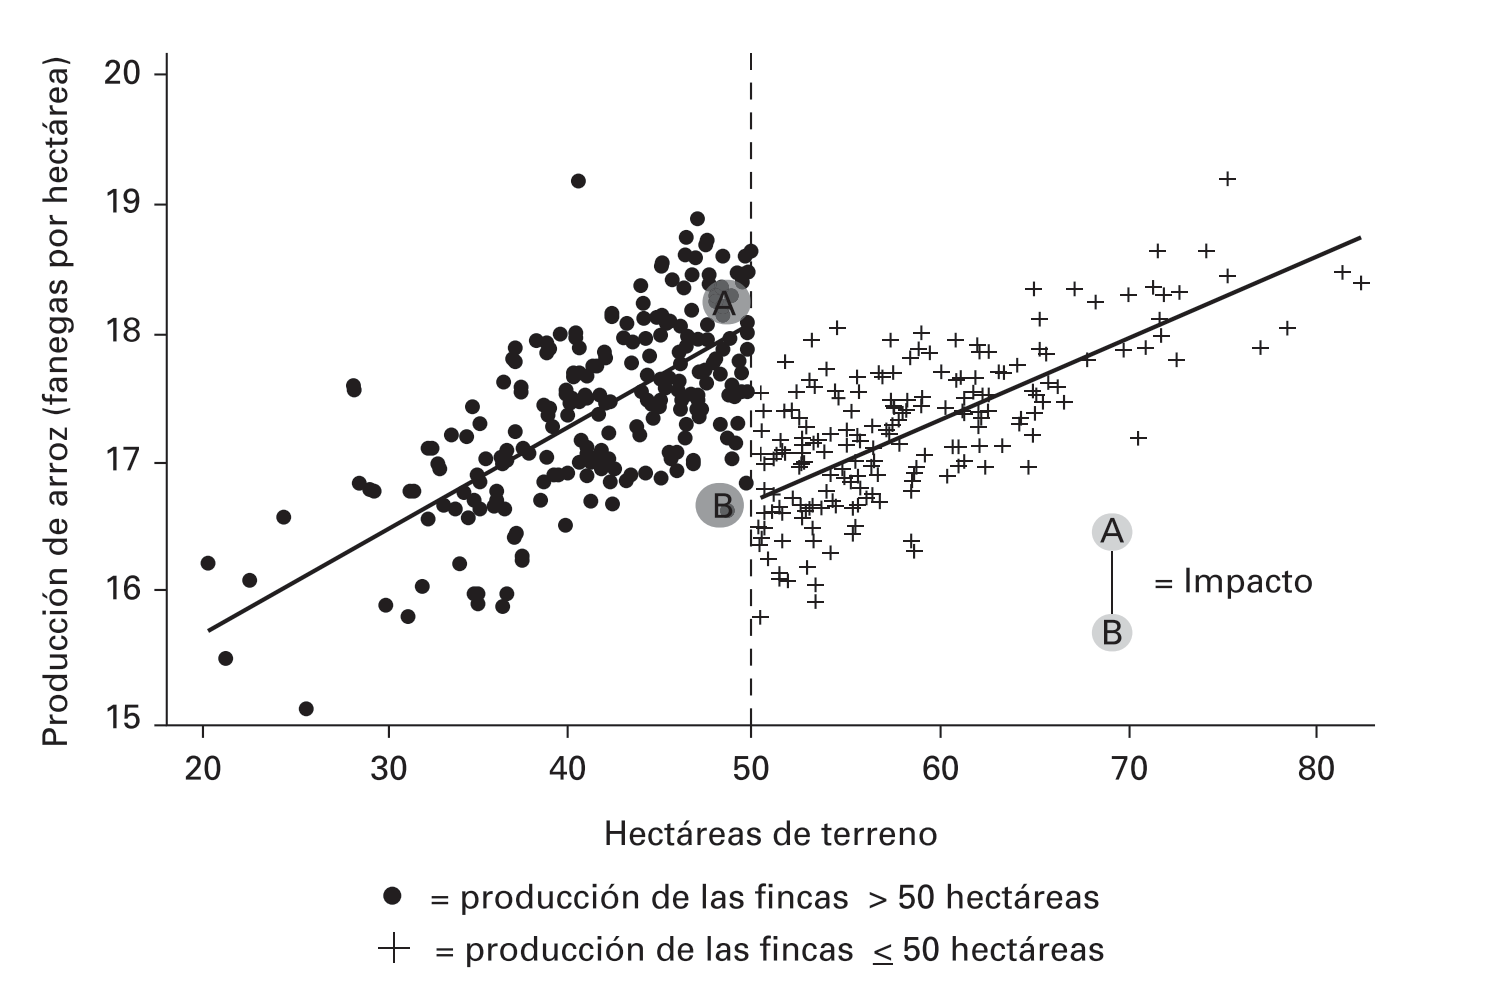
\includegraphics[width=0.9\textwidth,height=\textheight]{arroz2}
\end{frame}

\hypertarget{identificaciuxf3n}{%
\section{Identificación}\label{identificaciuxf3n}}

\begin{frame}{Identificación}
\protect\hypertarget{identificaciuxf3n-1}{}
Identificación no paramétrica en RD:

Suponemos:

\begin{enumerate}
\tightlist
\item
  diseño ``nítido'' (\emph{sharp}): \(T_i = 1(X_i >= c)\)
\item
  (suavidad): \(E[Y_{i0}|X_i=x], E[Y_{i1}|X_i=x]\) es continuo en
  \(x=c\)
\end{enumerate}

Por tanto,

\[E[\tau_i|X_i = c] = \lim_{x \downarrow  c}E[Y_i|X_i=x]-\lim_{x \uparrow  c}E[Y_i|X_i=x]\]
\end{frame}

\begin{frame}{Identificación}
\protect\hypertarget{identificaciuxf3n-2}{}
Diferencia de medias (\emph{naive}) tiene el mismo sesgo de selección en
la estimación del efecto que vimos en clases anteriores cuando hay
\emph{confounders}.

\[
\begin{aligned}
\Delta(h) &= E\{Y_i | X_i \in [c, c+h]\} - E\{Y_i | X_i \in [c-h, h]\} \\
          &= E\{Y_{(1)} | X_i \in [c, c+h]\} - E\{Y_{(0)} | X_i \in [c-h, h]\} \\ 
          &= E\{\tau | X_i \in [c, c+h]\} + Bias(h)
\end{aligned}
\] donde
\[Bias(h) = E\{Y_{(0)} | X_i \in [c, c+h]\} - E\{Y_{(0)} | X_i \in [c-h, h]\}\]

\begin{itemize}
\tightlist
\item
  Si ocurre que \(E[Y_{i(t)}|X_i=x]\) es continuo en x=c para \(t=0,1\),
\end{itemize}

\[\lim_{h \downarrow  0}\delta (h) = E[ \tau_i | X_i = c] \]
\end{frame}

\hypertarget{estimaciuxf3n-e-inferencia}{%
\section{Estimación e inferencia}\label{estimaciuxf3n-e-inferencia}}

\begin{frame}{Estimación}
\protect\hypertarget{estimaciuxf3n}{}
\begin{itemize}
\tightlist
\item
  Estimar funciones de regresión a la izquierda y a la derecha del punto
  de corte \pause
\item
  Global:

  \begin{itemize}
  \tightlist
  \item
    Estimar un polinomio de orden \emph{p} en toda la muestra
  \item
    Sensible a errores de especificación
  \item
    Comportamiento errático en los puntos de corte \pause
  \end{itemize}
\item
  ``Paramétrico flexible'':

  \begin{itemize}
  \tightlist
  \item
    Estimar un polinomio dentro de un ancho de banda \emph{ad-hoc}
    \pause
  \end{itemize}
\item
  Polinomio local:

  \begin{itemize}
  \tightlist
  \item
    Selección de ancho de banda basada en datos, no paramétrica
  \item
    Tiene en cuenta problemas de especificación al realizar inferencias
  \end{itemize}
\end{itemize}
\end{frame}

\begin{frame}{Estimación global}
\protect\hypertarget{estimaciuxf3n-global}{}
\[E[Y_{i(t)}|X_i] = \alpha_t + \beta_t(X_i - c)\]
\end{frame}

\begin{frame}{Estimación global (orden 0)}
\protect\hypertarget{estimaciuxf3n-global-orden-0}{}
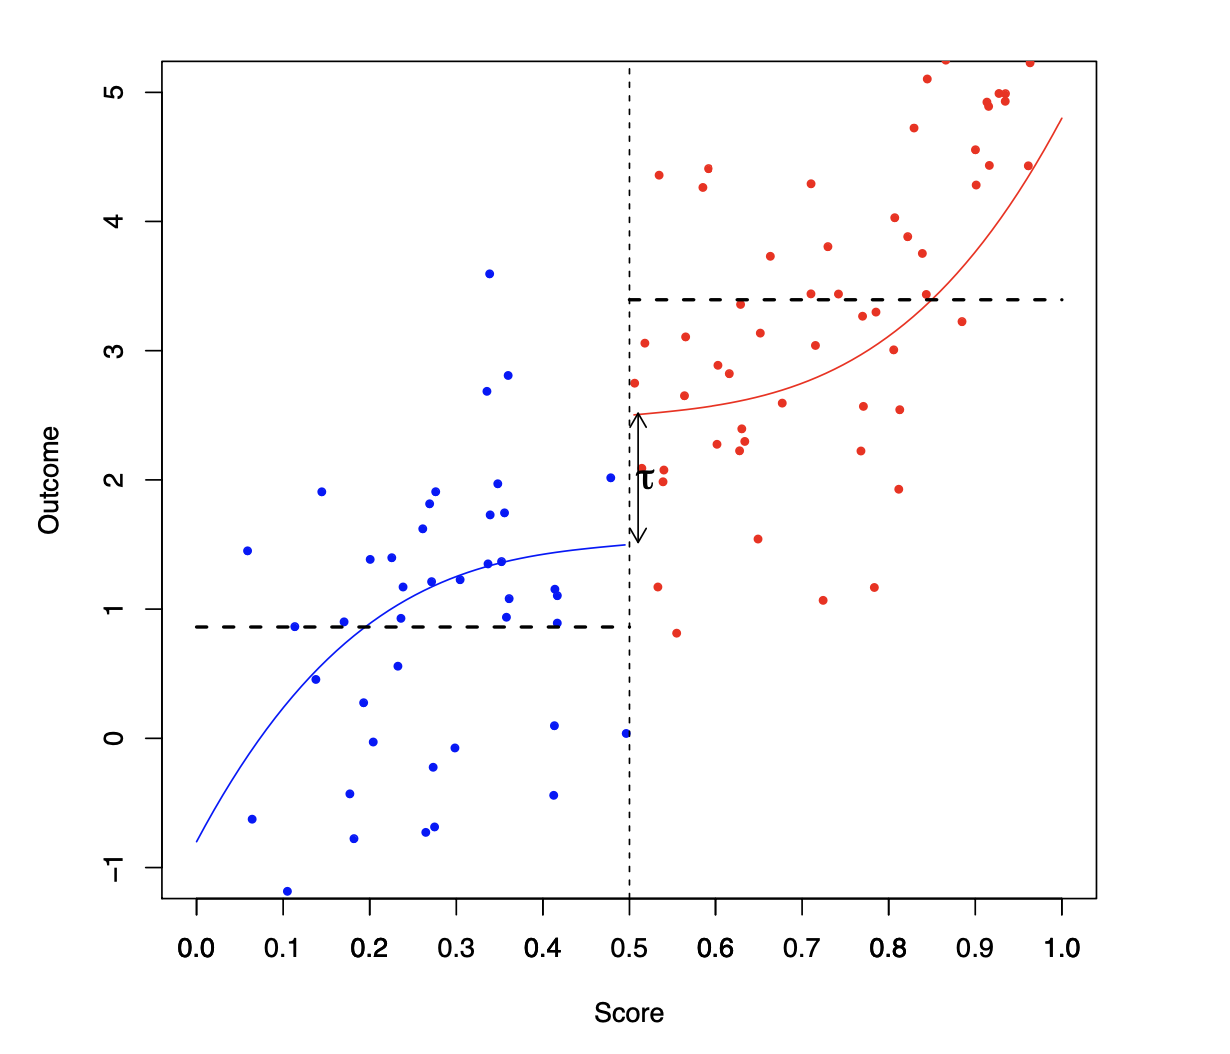
\includegraphics[width=0.9\textwidth,height=\textheight]{p0}
\end{frame}

\begin{frame}{Estimación global (orden 1)}
\protect\hypertarget{estimaciuxf3n-global-orden-1}{}
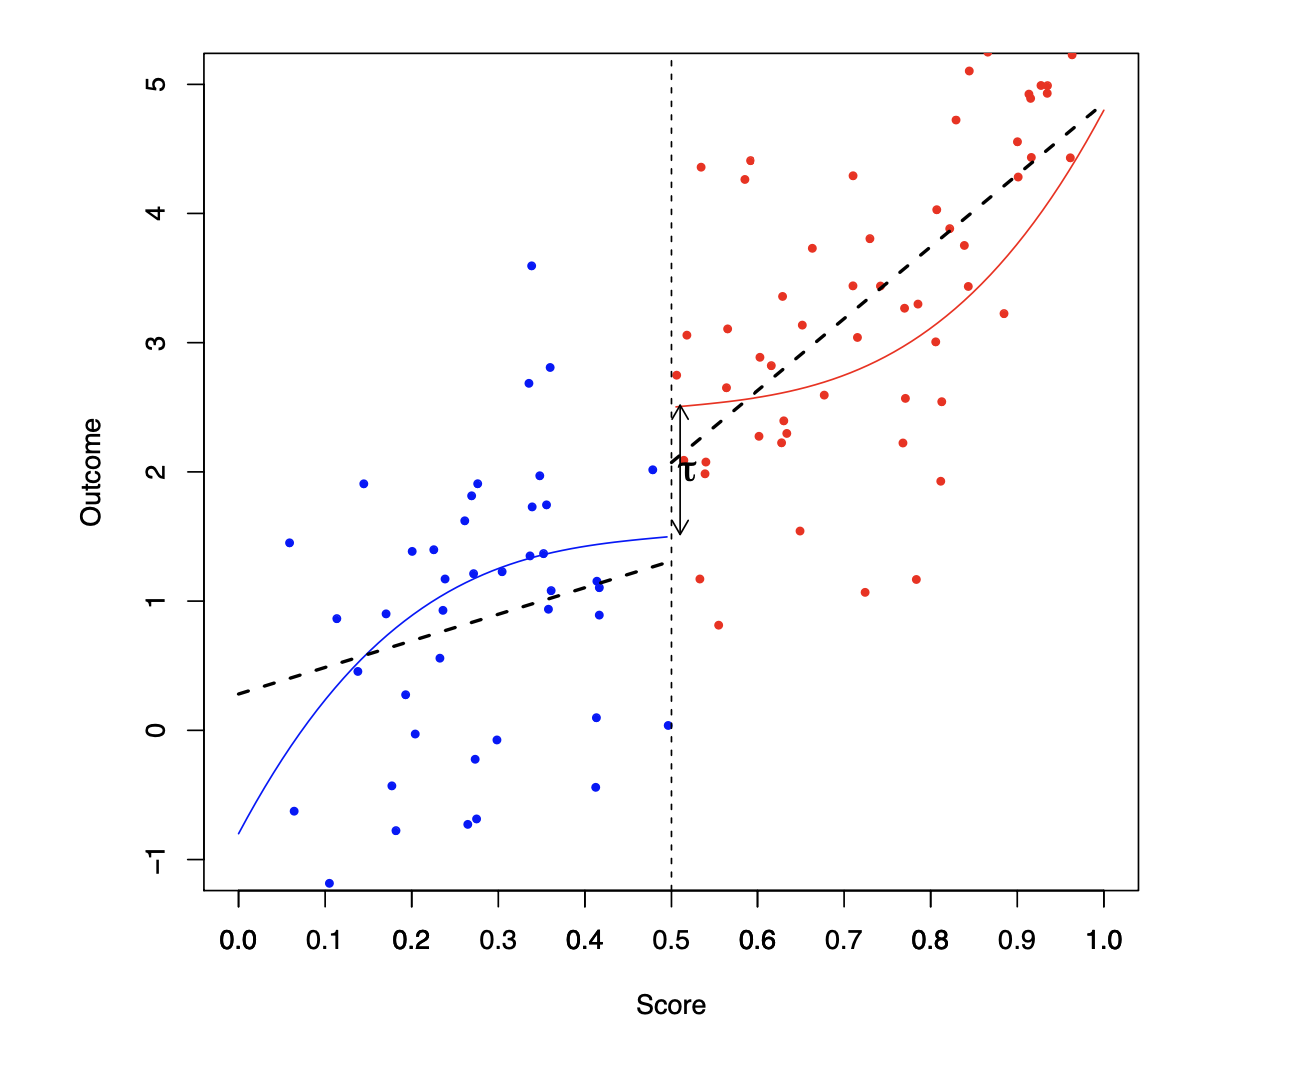
\includegraphics[width=0.9\textwidth,height=\textheight]{p1}
\end{frame}

\begin{frame}{Estimación global (orden 2)}
\protect\hypertarget{estimaciuxf3n-global-orden-2}{}
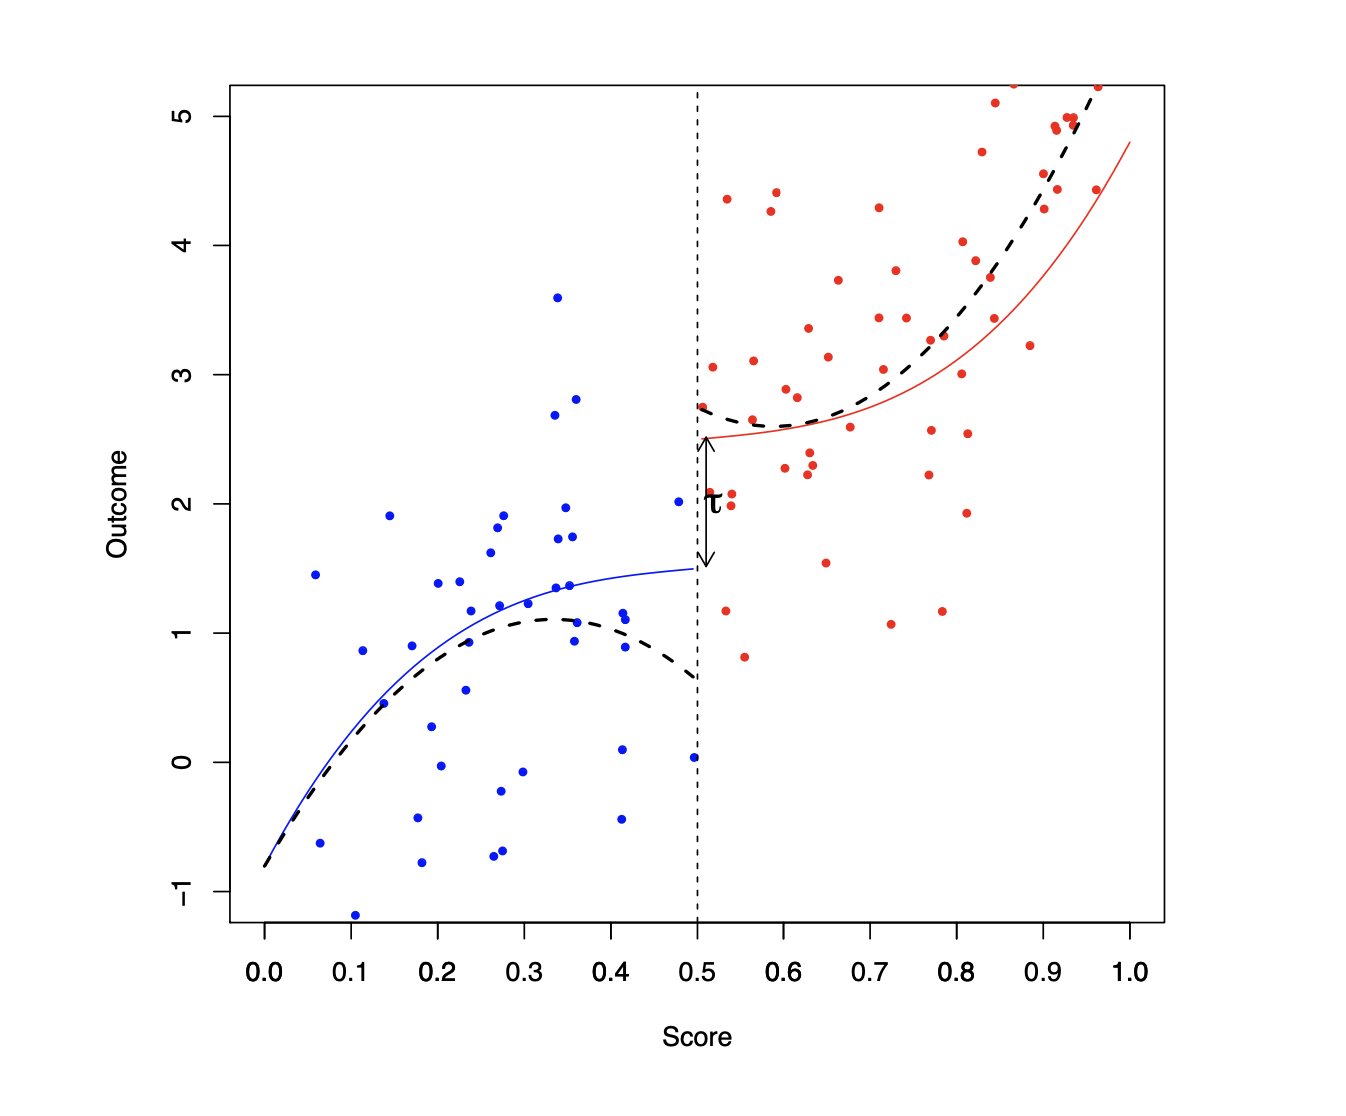
\includegraphics[width=0.9\textwidth,height=\textheight]{p2}
\end{frame}

\begin{frame}{Estimación global (orden 3)}
\protect\hypertarget{estimaciuxf3n-global-orden-3}{}
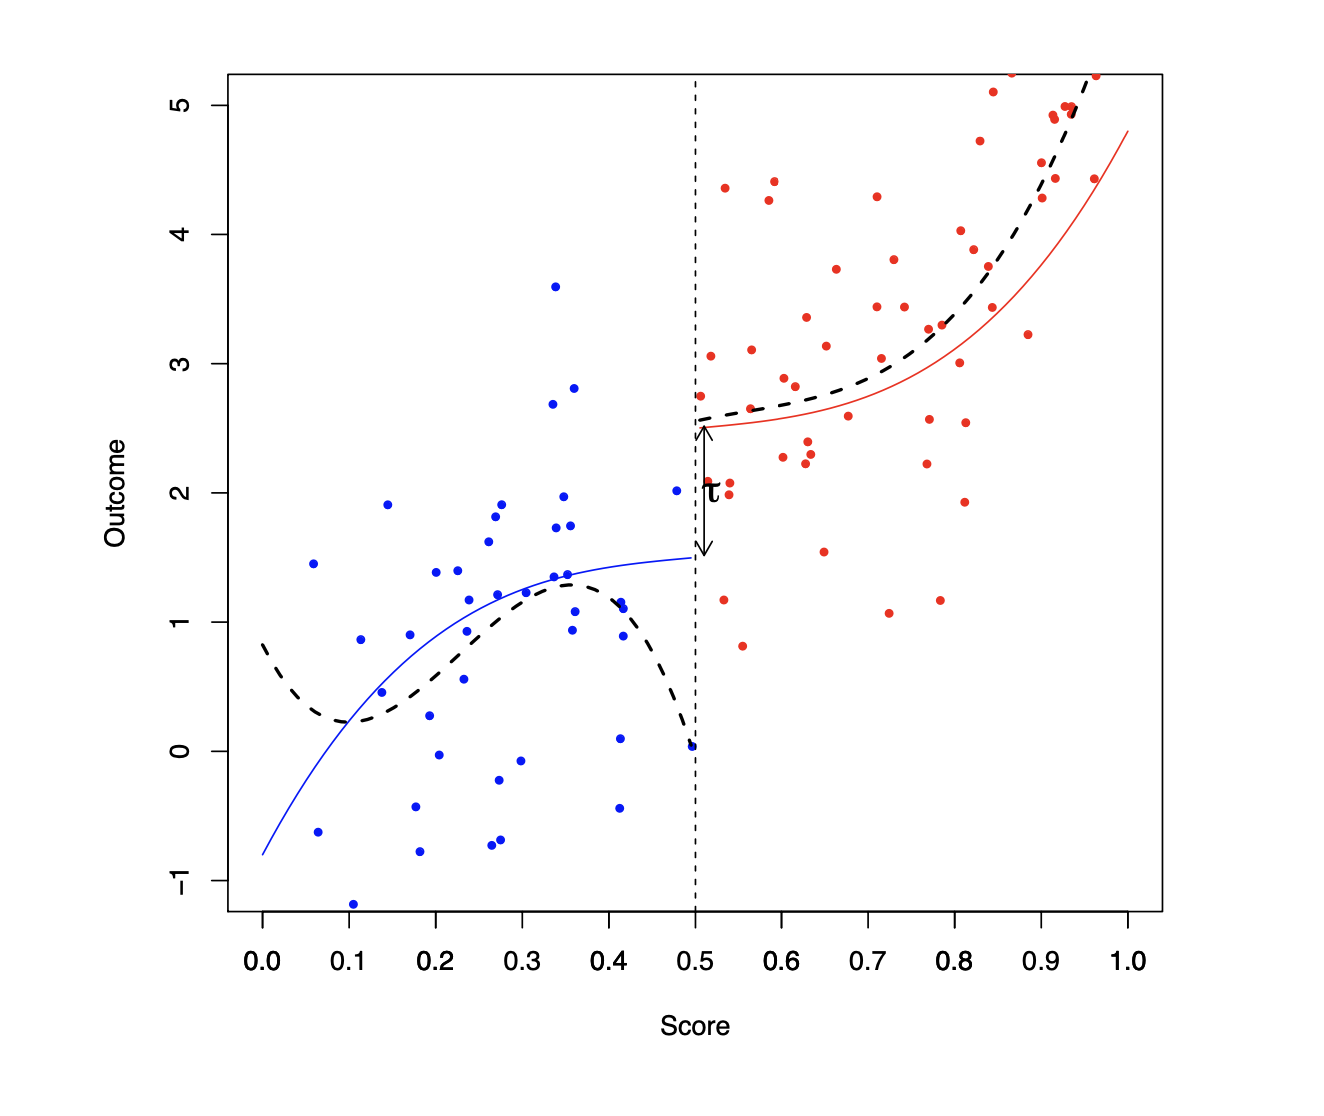
\includegraphics[width=0.9\textwidth,height=\textheight]{p3}
\end{frame}

\begin{frame}{Estimación local}
\protect\hypertarget{estimaciuxf3n-local}{}
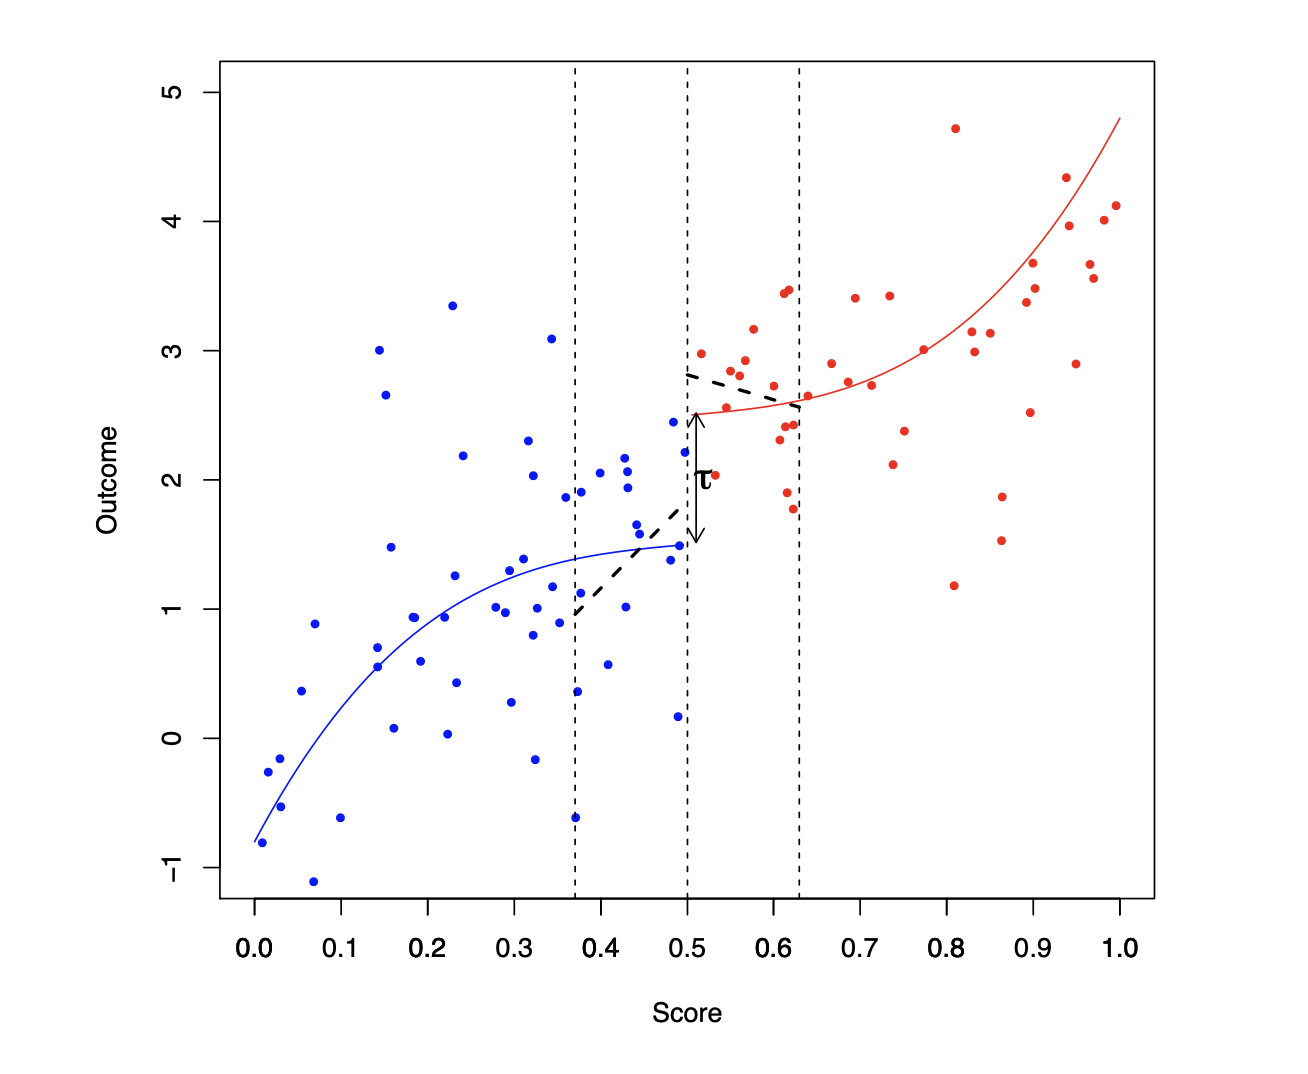
\includegraphics[width=0.9\textwidth,height=\textheight]{llr}
\end{frame}

\begin{frame}{Estimación local}
\protect\hypertarget{estimaciuxf3n-local-1}{}
\begin{itemize}
\tightlist
\item
  Estimación no paramétrica debe dar cuenta del sesgo
\item
  Si \(h=0\), el estimador es insesgado
\item
  Pero \(h=0\) implica que no hay observaciones dentro de la ventana
\item
  Menor \(h\) implica un pequeño sesgo, pero menos observaciones (mayor
  varianza)
\item
  \emph{Optimal bandwith}
\end{itemize}
\end{frame}

\hypertarget{ejemplos}{%
\section{Ejemplos}\label{ejemplos}}

\begin{frame}{Ejemplo gráfico}
\protect\hypertarget{ejemplo-gruxe1fico}{}
Programa nutricional para niños de 5-9 años.
\end{frame}

\begin{frame}{Ejemplo gráfico}
\protect\hypertarget{ejemplo-gruxe1fico-1}{}
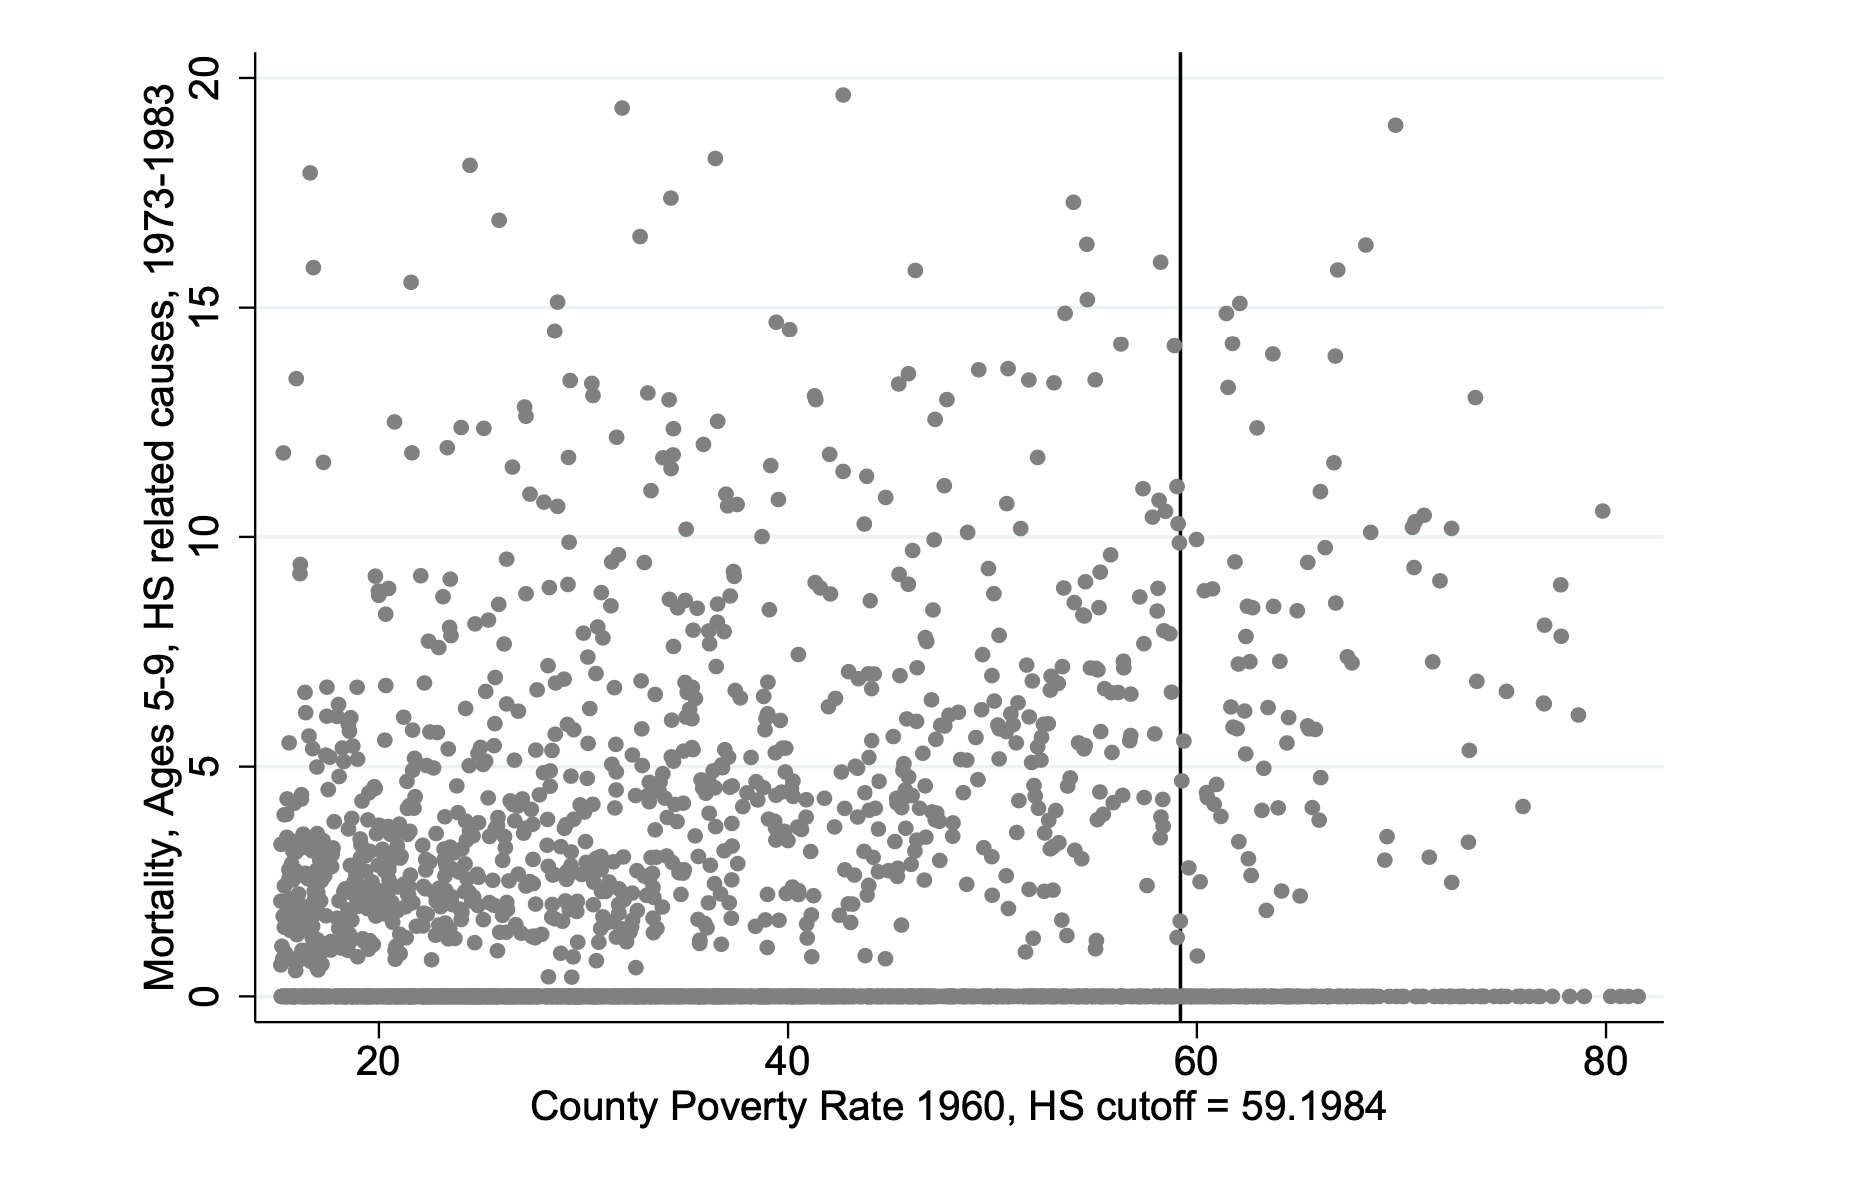
\includegraphics[width=0.9\textwidth,height=\textheight]{ej1}
\end{frame}

\begin{frame}{Ejemplo gráfico}
\protect\hypertarget{ejemplo-gruxe1fico-2}{}
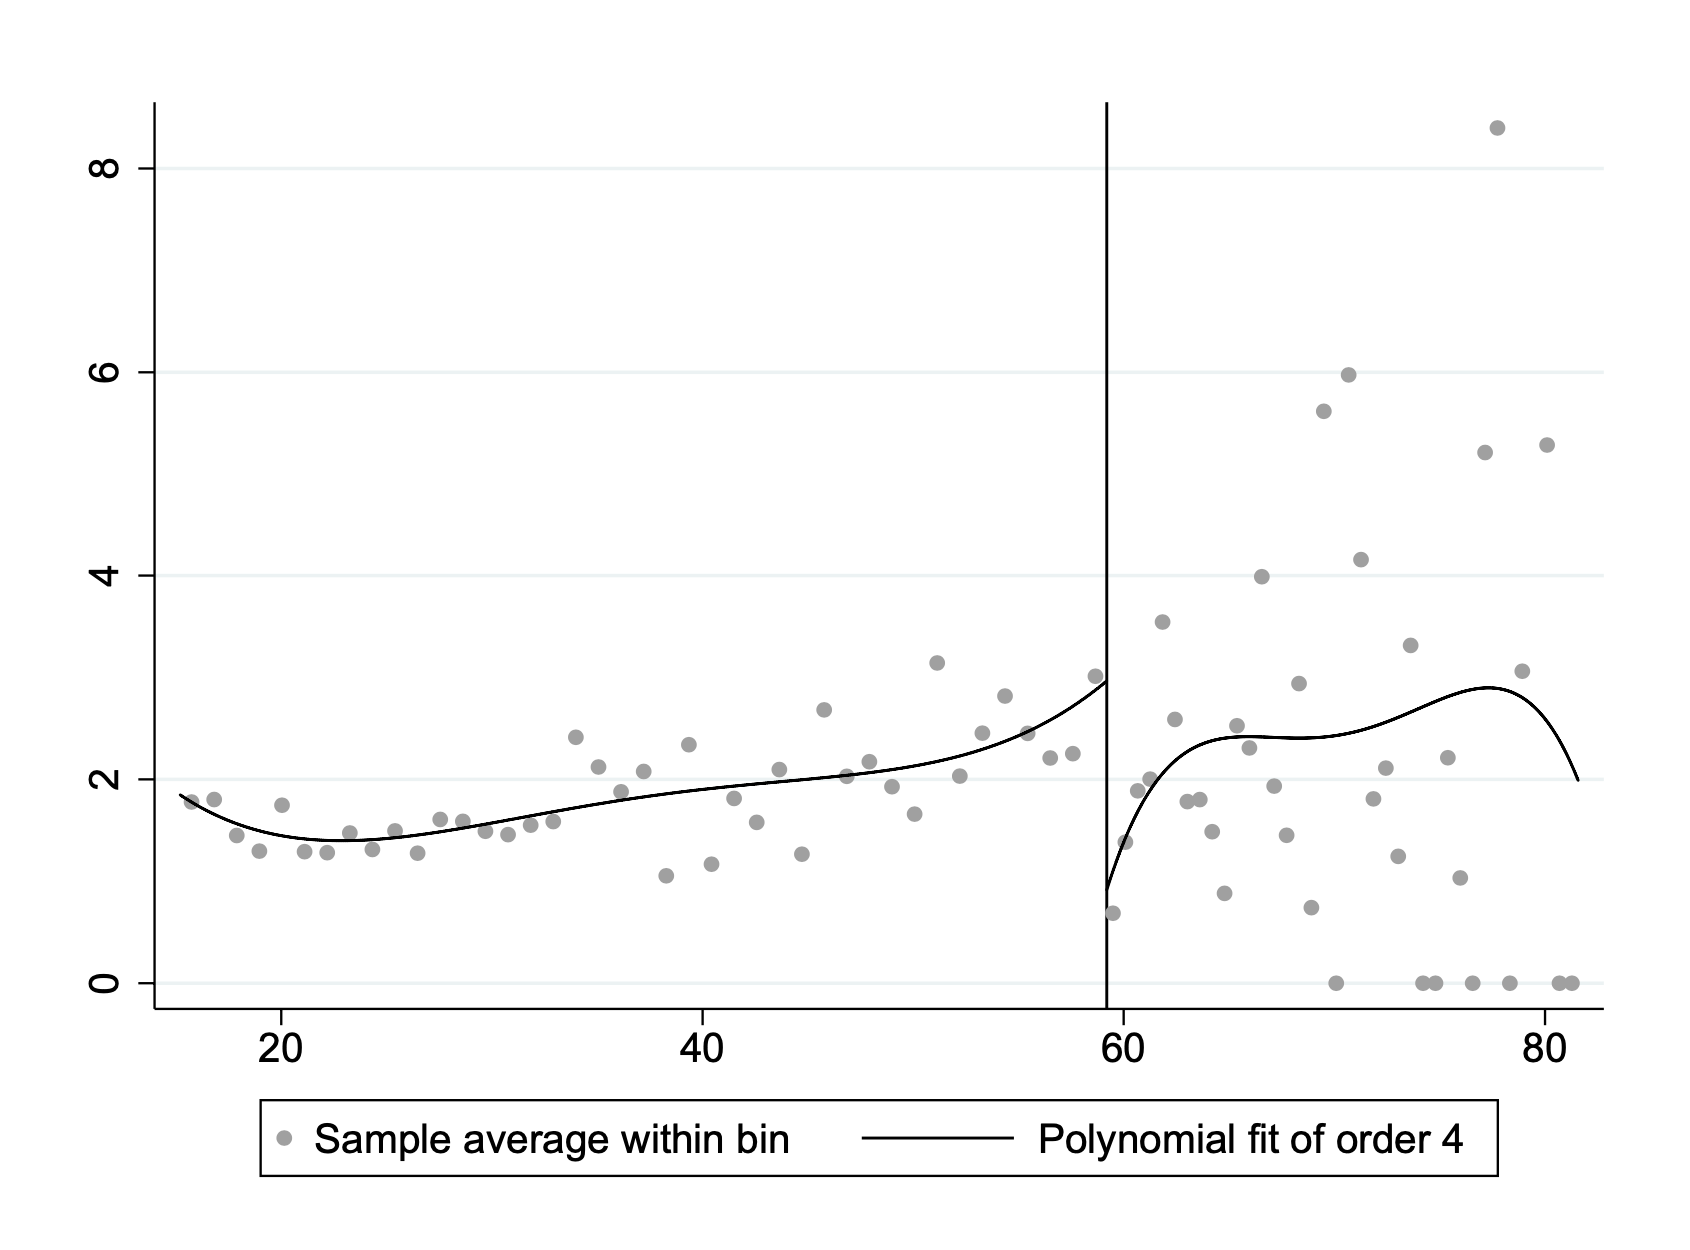
\includegraphics[width=0.9\textwidth,height=\textheight]{ej2}
\end{frame}

\begin{frame}{Ejemplo gráfico}
\protect\hypertarget{ejemplo-gruxe1fico-3}{}
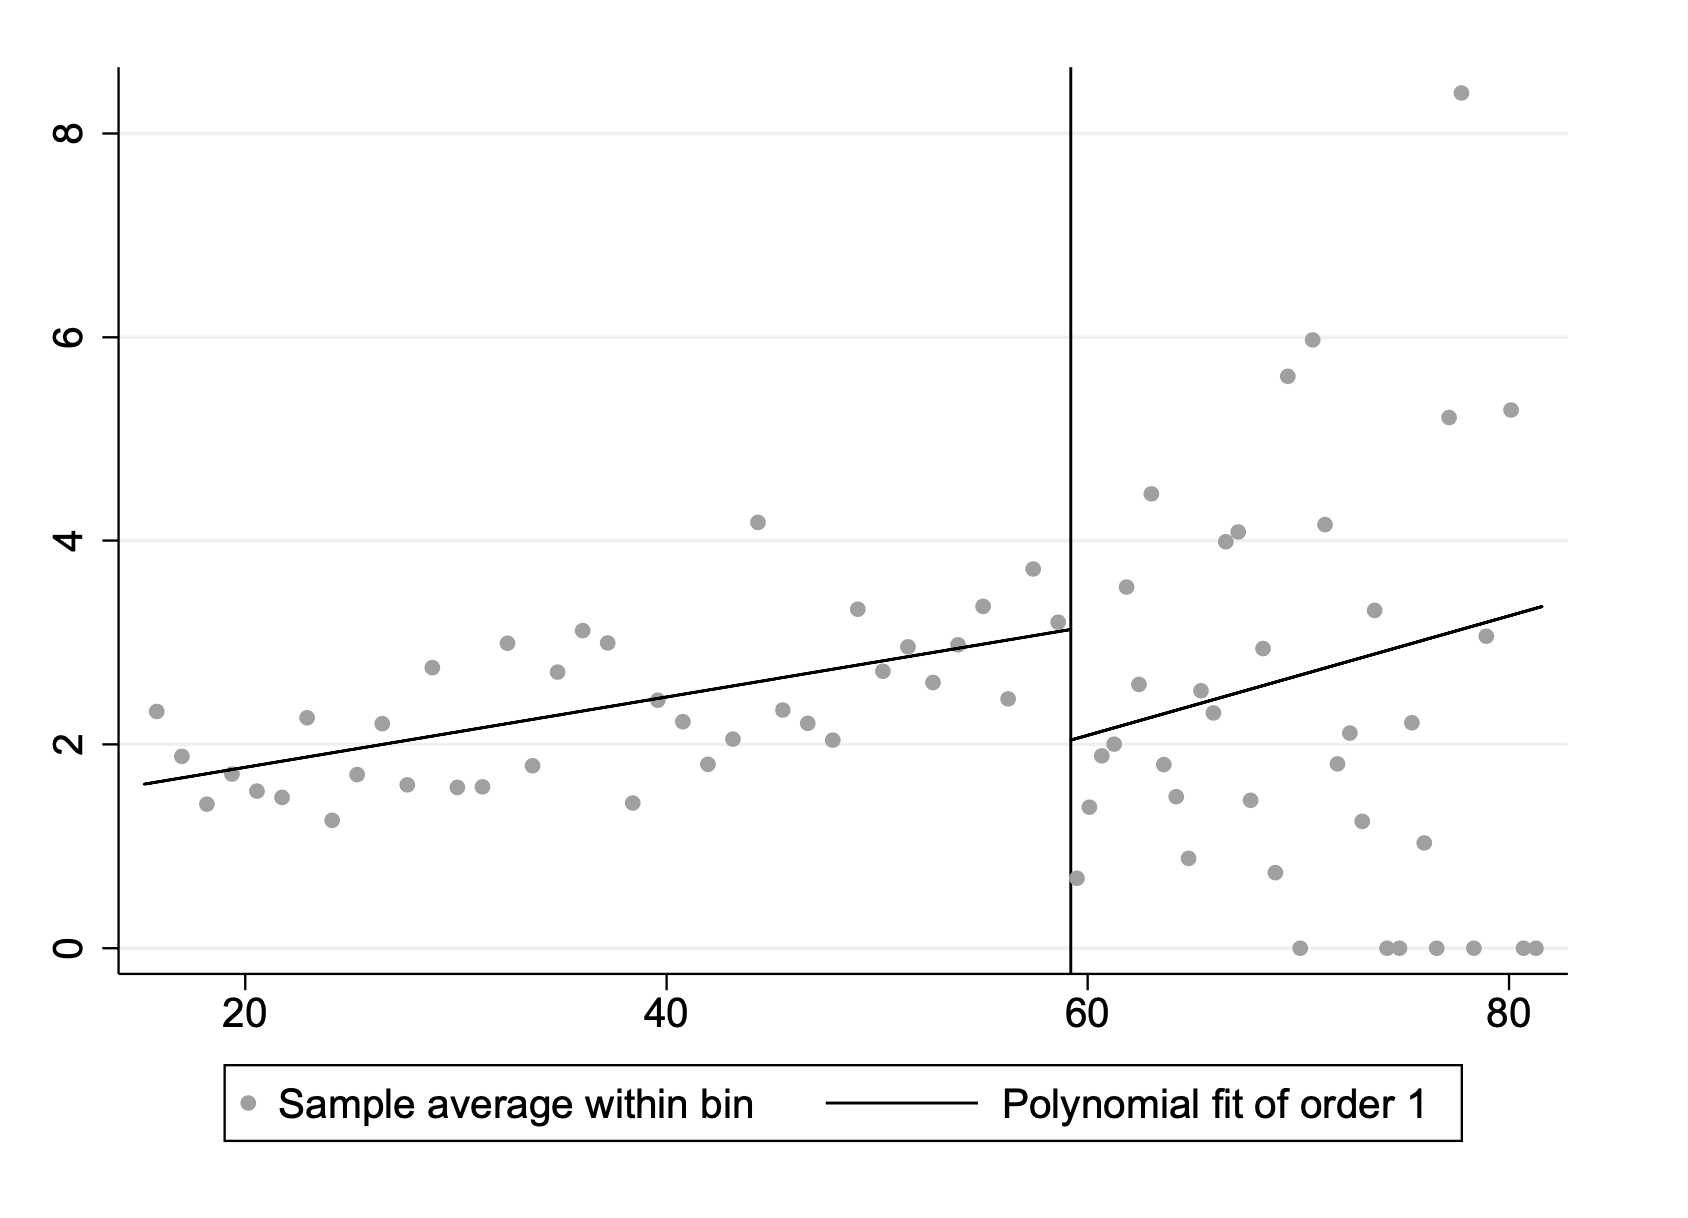
\includegraphics[width=0.9\textwidth,height=\textheight]{ej3}
\end{frame}

\hypertarget{diseuxf1o-difuso}{%
\section{Diseño difuso}\label{diseuxf1o-difuso}}

\begin{frame}{(Fuzzy) DRD}
\protect\hypertarget{fuzzy-drd}{}
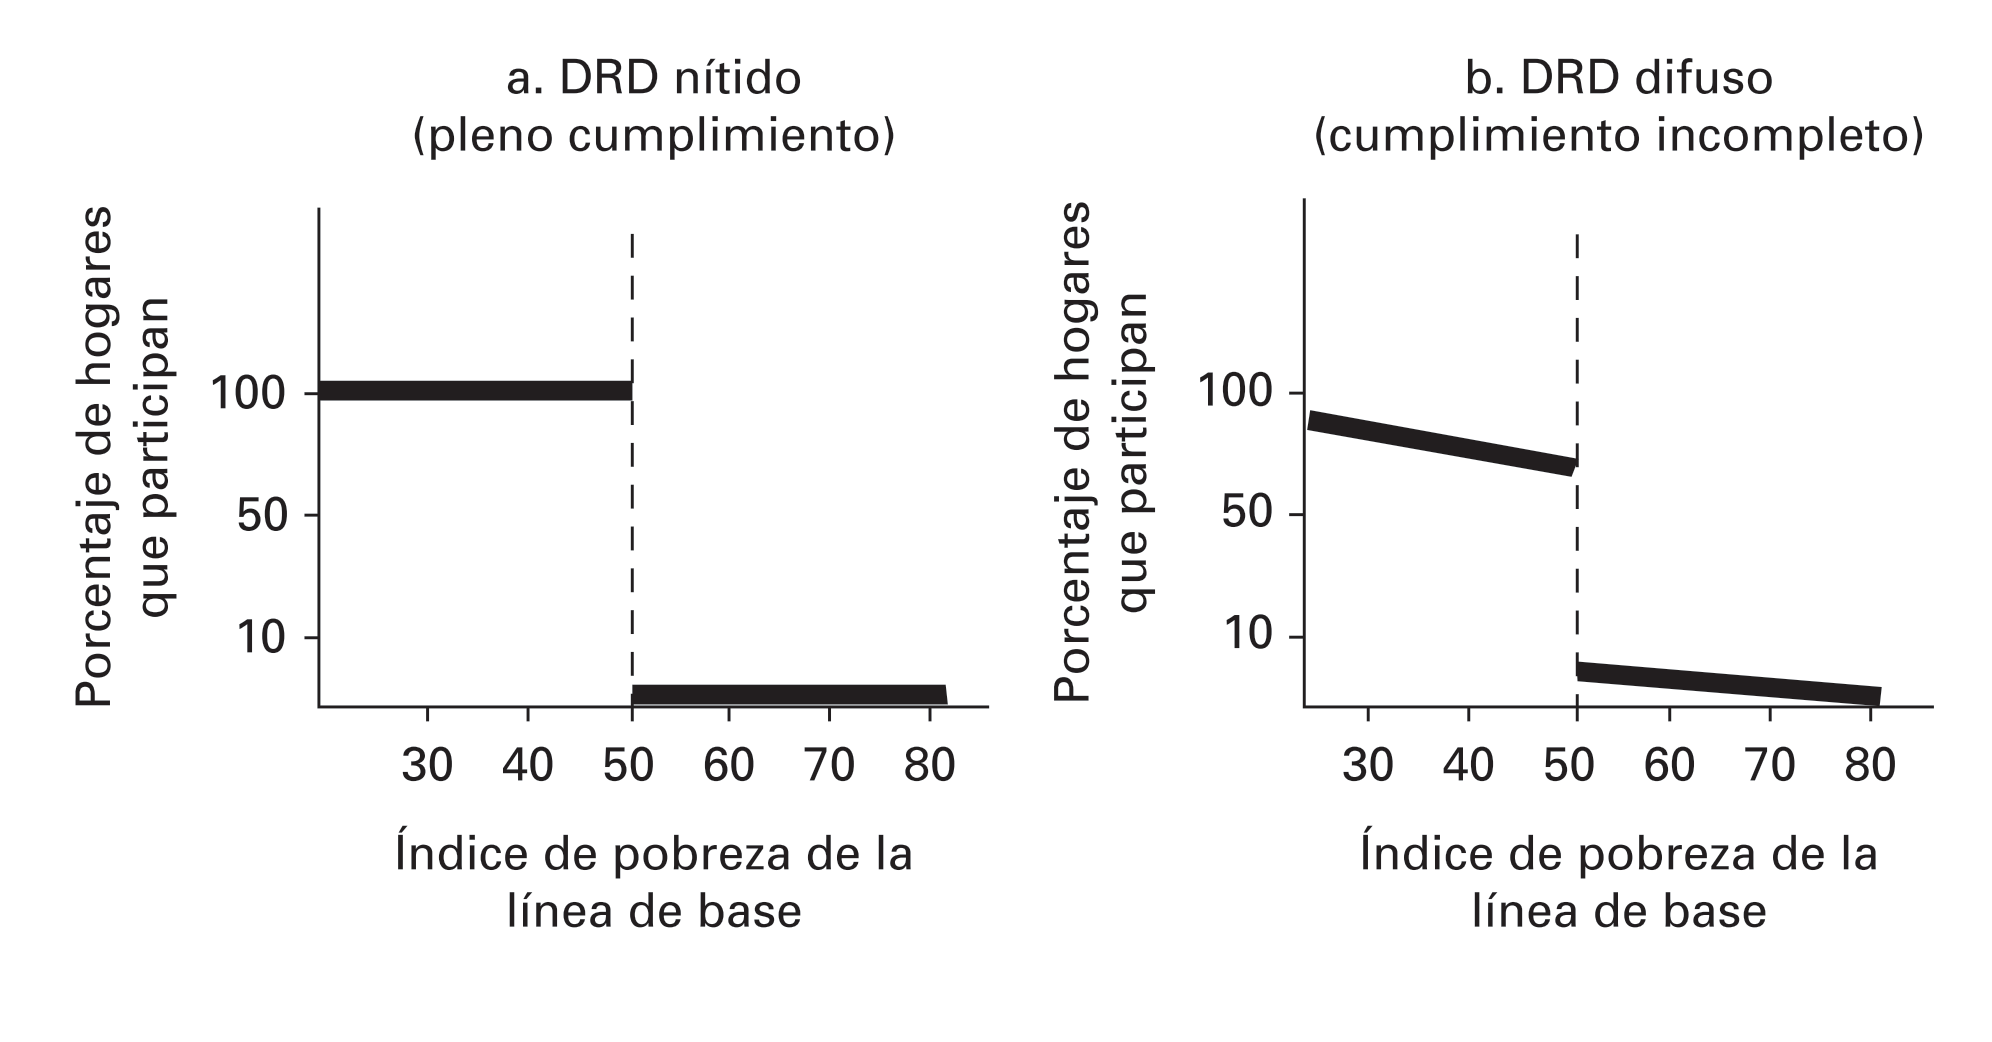
\includegraphics[width=0.9\textwidth,height=\textheight]{fuzzy_ejemplo}
\end{frame}

\hypertarget{chequeos-y-validez}{%
\section{Chequeos y validez}\label{chequeos-y-validez}}

\begin{frame}{Chequeos y validez}
Es importante que el índice de elegibilidad no sea manipulado en la
cercanía de la puntuación límite

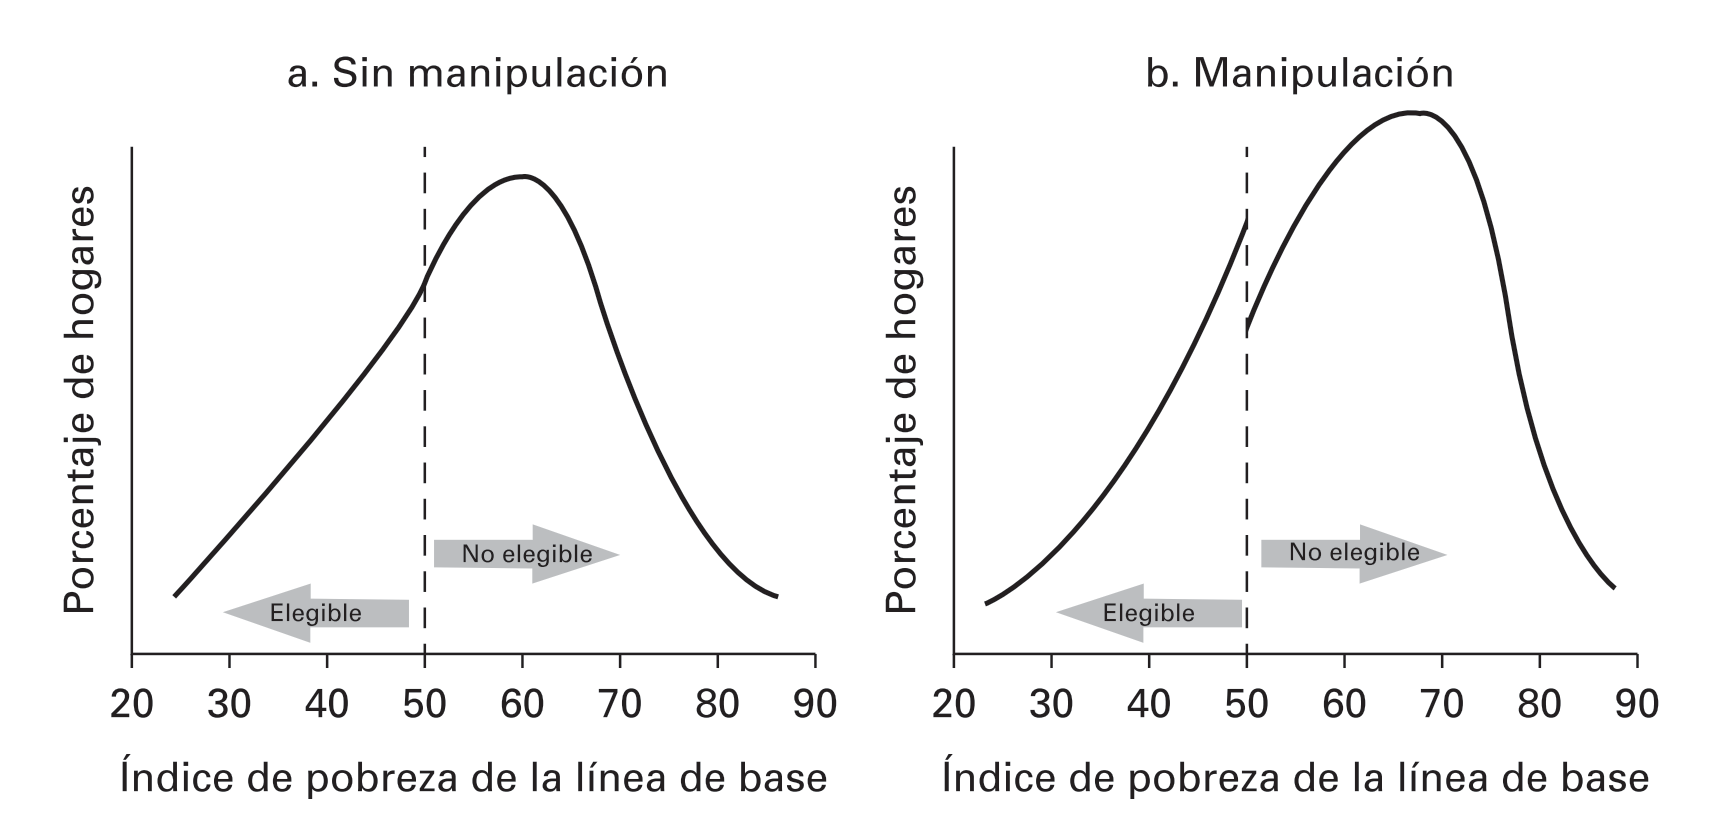
\includegraphics[width=0.9\textwidth,height=\textheight]{manipulacion}
\end{frame}

\begin{frame}{Lista de verificación}
\protect\hypertarget{lista-de-verificaciuxf3n}{}
\begin{itemize}
\item
  ¿Es continuo el índice en torno la puntuación límite en el momento de
  la línea de base? \pause
\item
  ¿Hay alguna evidencia de falta de cumplimiento de la regla que
  determine la elegibilidad para el tratamiento?

  \begin{itemize}
  \tightlist
  \item
    Compruébese que todas las unidades elegibles y ninguna unidad no
    elegible han recibido el tratamiento.
  \item
    Si se encuentra falta de cumplimiento, habrá que combinar el DRD con
    un enfoque de variable instrumental para corregir esta
    \emph{discontinuidad difusa}.\footnote<.->{Se utiliza la
      localización a la izquierda o la derecha del punto de corte como
      variable instrumental para la aceptación del programa en la
      primera etapa de una estimación de mínimos cuadrados en dos
      etapas.}
  \end{itemize}
\end{itemize}
\end{frame}

\begin{frame}{Lista de verificación}
\protect\hypertarget{lista-de-verificaciuxf3n-1}{}
\begin{itemize}
\tightlist
\item
  ¿Hay alguna evidencia de que las puntuaciones del índice puedan haber
  sido manipuladas con el fin de influir en quien tenía derecho a
  beneficiarse del programa?

  \begin{itemize}
  \tightlist
  \item
    Compruébese si la distribución de la puntuación del índice es fluida
    en el punto límite.
  \item
    Si se halla evidencia de una \emph{concentración} de puntuaciones ya
    sea por encima o por debajo del punto límite, puede que esto sea una
    señal de manipulación. \pause
  \end{itemize}
\item
  ¿El umbral corresponde a un único programa que se está evaluando o
  está siendo usado por otros programas también?
\end{itemize}
\end{frame}

\hypertarget{anuxe1lisis-estaduxedstico-de-drd}{%
\section{Análisis estadístico de
DRD}\label{anuxe1lisis-estaduxedstico-de-drd}}

\begin{frame}[fragile]{\(\textbf{R}\)}
\protect\hypertarget{textbfr}{}
\texttt{rdrobust}: graphical presentation and local polynomial methods

\texttt{rddensity}: density discontinuity tests (manipulation testing)

\texttt{rdlocrand}: local randomization methods

\texttt{rdmulti}: analysis of RD with multiple cutoffs or scores

\texttt{rdpower}: power and sample size calculation
\end{frame}

\end{document}
